

\section{Introdução}

O presente relatório tem como objetivo descrever todo o processo implementado durante a resolução do segundo trabalho prático da UC de Processamento de Linguagem Natural.

O trabalho em causa tem como objetivo a criação de uma ferramenta de visualização dos dados, previamente em formato JSON, decorrentes dos PDFs selecionados no trabalho prático anterior.

Com isto, pretende-se enriquecer todos os conjuntos de dados a utilizar, através da adição de novas informações, provenientes de fontes externas, como \textit{websites}, ou outros dicionários relacionados com o tema em causa. Além disso, será estabelecida uma análise minuciosa dos conceitos anteriormente extraídos, de maneira a serem identificadas eventuais relações, ou novos agrupamentos por categorias. Assim, a ferramenta final desenvolvida tem a capacidade de explorar as relações presentes entre determinados termos.


Por conseguinte, neste relatório, será inicialmente explorado todo o processo de \textit{Web Scraping} implementado para os três conjuntos de dados a serem utilizados, essencial para a obtenção das descrições dos demais conceitos, e, ainda, para a obtenção de novos termos, oriundos de novos dicionários \textit{online}.
Posteriormente, será exemplificado todo o processo envolvido no desenvolvimento da plataforma \textit{web}, bem como uma descrição e demonstração das suas funcionalidades.

\section{Tarefas}

Tal como é possível averiguar na Introdução, o presente projeto envolve duas tarefas globais:
\begin{itemize}
    \item \textbf{Enriquecer os \textit{datasets}}: Por forma a enriquecer a informação contida na ferramenta final, é recomendada a extração de novos conceitos, ou, ainda, a adição de novos atributos como sinónimos, definições, termos relacionados ou categorias dos termos já existentes. Assim, para este processo será implementado um \textit{Web Scraping} a partir de fontes externas, como dicionários médicos, \textit{websites} ou outras fontes relevantes.

    \item \textbf{Plataforma \textit{Web}}: Como passo final, será desenvolvida uma plataforma \textit{web}, através da \textit{framework} \textbf{Flask}, que permita representar e manipular os \textit{datasets} em causa. Esta terá diferentes funcionalidades como a adição de novas informações ao conjunto de dados, eliminação de determinados termos, ou, ainda, atualização das informações já existentes.
\end{itemize}

\section{Web Scraping}

Antes de mais, é importante relembrar os conjuntos de dados que foram obtidos com a realização do primeiro trabalho prático da Unidade Curricular:

\begin{itemize}
    \item \textbf{Glossário do Ministério da Saúde}: O documento em causa trata-se de um glossário composto por vocabulário controlado, e de qualidade, onde podem ser verificadas 4 secções:
    \begin{itemize}
        \item Siglas: Secção com uma lista de siglas utilizadas ao longo do documento;

        \item Glossário: Secção maioritária do documento, composta pelos termos e o seu significado, bem como a(s) categoria(s) a que cada termo pertence;

        \item Áreas temáticas: Secção com todas as categorias referidas ao longo do glossário, bem como a sua definição;

        \item Termos organizados por categoria: Nesta secção, para cada categoria, verifica-se uma lista dos termos que a mesma engloba.
    \end{itemize}
  
    
    \item \textbf{Anatomia na Prática - Sistema Musculoesquelético}: Para este PDF procedeu-se à obtenção de um dicionário com duas chaves principais: \textit{Sistema Esquelético e Articular} e \textit{Sistema Muscular}. Cada uma destas assume como valor um novo dicionário cujas chaves se referem à secção em análise, isto é, Crânio, Membro Inferior, Membro Superior, etc. Por sua vez, cada secção verifica como valor um outro dicionário cujas chaves correspondem à subsecção em análise, como Crânio: Vista Anterior - I. Assim, cada subsecção apresenta como valor uma lista dos demais termos associados.
    É importante notar que cada subsecção pode verificar, ainda, uma secção interior, sendo que é nesta última que se observa a lista das terminologias.
    
\end{itemize}

É importante notar que todo o processo de \textit{Web Scraping} foi conseguido graças à biblioteca \textit{BeautifulSoup}, um pacote \textit{Python} específico para a análise de documentos \textit{HTML} e \textit{XML}, uma vez que procede à criação de uma árvore de análise que pode ser utilizada para extrair dados, sendo extremamente útil para o processo em causa \cite{BSoup2024}. \\
Para além disso, esta ferramenta foi utilizada em conjunto com a biblioteca \textit{requests}, que permite o envio de pedidos \textit{HTTP}, onde cada um retorna um objeto com todos os dados de resposta (conteúdo, codificação, etc) \cite{Requests2024}.

\subsection{Web Scraping - Anatomia na Prática}

Em relação ao documento Anatomia na Prática, procedeu-se à obtenção das descrições dos vários ossos em análise, bem como dos vários músculos, dado que se trata de um componente essencial para uma melhor compreensão da anatomia do corpo humano.

\textbf{Obtenção das descrições dos ossos:}\\
Para tal, devido à falta de dicionários médicos \textit{online}, específicos para o tema em questão, foi utilizada a \textit{Wikipedia} como fonte de informação, mais especificamente, a página referente à lista de ossos do corpo humano \cite{wikipedia2024ossos}.


A página em questão apresenta as demais nomenclaturas dos ossos do corpo humano organizadas por categorias, como, por exemplo: ossos do crânio, ossos da face, ossos do ouvido, etc, tendo sido bastante crucial para a obtenção dos diversos \textit{hiperlinks}, que permitem redirecionar para a página específica de cada osso, dado que é lá que se encontra a descrição do mesmo. 

Como passo inicial, procedeu-se ao estabelecimento de um pedido HTTP GET, através da biblioteca \textit{requests}, relativamente ao URL da página anteriormente referida. Posteriormente, procedeu-se à conversão do conteúdo HTML da resposta num objeto \textit{BeautifulSoup}, por forma a facilitar a navegação e extração de dados.

Dado por implementado o objeto anunciado, foi inicializada uma lista, designada por \textit{url\_pages}, com o objetivo de armazenar os valores dos atributos \textit{href}, dos elementos âncora, uma vez que denotam um \textit{hiperlink} de um endereço da \textit{web} para outro.

É importante referir que, como as várias nomenclaturas são disponibilizadas por tópicos, constituintes de uma lista, os elementos âncora a procurar, fazem todos parte de um determinado elemento \textit{li}, ou seja, de um item de lista.

Assim, dado por obtidos os demais elementos \textit{li}, através da função \textit{find\_all}, caracterizados por não possuírem qualquer \textit{id}, ou classe, os mesmos foram percorridos de maneira a serem acedidos os valores dos atributos \textit{href} dos elementos âncora. 

\begin{figure}[H]
    \centering
    \centering
    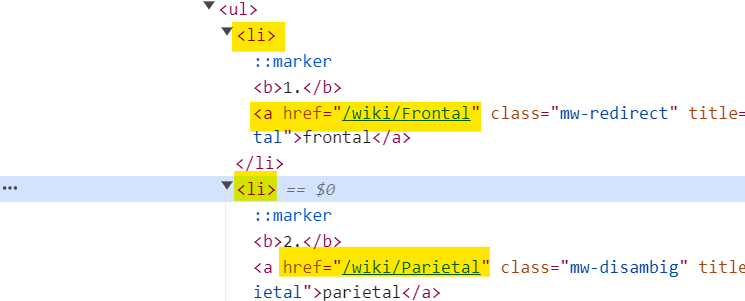
\includegraphics[width=0.6\textwidth]{Images/web1.png}
    \caption{Elementos âncora}
    \label{fig:dic-traduc1}
\end{figure}

Assim, foi possível proceder à definição dos \textit{links} de cada uma das páginas específicas, através da concatenação entre a \textit{string} \textit{https://pt.wikipedia.org}, e o valor de cada atributo \textit{href}, tendo sido estes armazenados na lista anteriormente definida.

Por sua vez, a lista em questão foi percorrida, de maneira a serem acedidas todas as páginas dos ossos em questão. Este processo foi bastante semelhante ao descrito anteriormente, ou seja, através do estabelecimento de um pedido HTTP GET, e posterior criação de um objeto \textit{BeautifulSoup}.

Uma vez aberta uma determinada página, foi estabelecida a obtenção do texto contido entre as \textit{tags} do primeiro parágrafo encontrado, envolvidas pelo elemento \textit{div} de classe \textit{mw-parser-output}, dado que corresponde à descrição desejada.

\begin{figure}[H]
    \centering
    \centering
    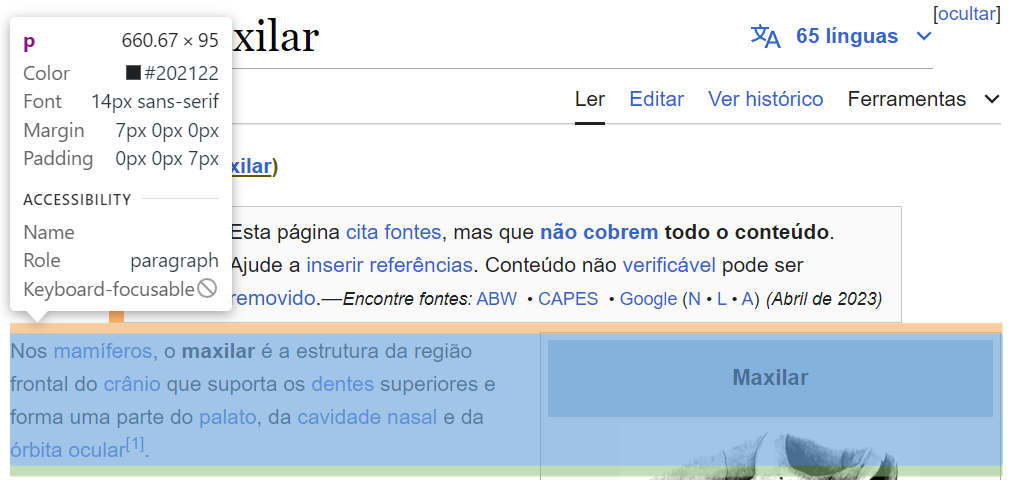
\includegraphics[width=0.6\textwidth]{Images/web2.png}
    \caption{Descrição correspondente ao osso maxilar \cite{wikipedia2024maxilar}}
    \label{fig:dic-traduc1}
\end{figure}

No entanto, durante este processo foram implementadas algumas operações de limpeza do texto, através do uso de expressões regulares.

Finalmente, foi criado um dicionário, designado \textit{ossos\_info}, que verifica, como chaves, as designações dos ossos em estudo, e, como valores, as descrições dos mesmos. Este foi posteriormente armazenado num ficheiro JSON.

\textbf{Obtenção das descrições dos músculos:}\\

Assim como foi realizado para os ossos, foi utilizada a página do Wikipedia com a lista dos músculos do corpo humano como fonte de informação \cite{wikipedia2024musculos}.

A página em questão apresenta as diferentes nomenclaturas dos músculos do corpo humano classificadas em categorias como, por exemplo, músculos da cabeça, músculos do tronco e músculos do membro superior. Para cada designação presente, a página disponibiliza um \textit{hiperlink} que direciona para a página específica de cada músculo, onde se encontra a descrição do mesmo.

Para a obtenção, portanto, das descrições, foi realizado, inicialmente, um pedido HTTP GET com uso da biblioteca \textit{requests}. Posteriormente, a fim de faciliar a navegação e a extração dos dados, foi realizada a conversão do conteúdo obtido num objeto \textit{BeautifulSoup}.

A partir da análise do conteúdo HTML obtido, foi possível identificar que as nomenclaturas estão situadas numa \textit{div} com classe \textit{my-body-content} e que são elementos de uma lista. Logo, através dos métodos \textit{find\_all} e \textit{find}, foi possível obter o parâmetro \textbf{href} dos elementos âncora que correspondem aos diferentes músculos. 

Com os parâmetros \textbf{href} obtidos, foram realizados novamente pedidos HTTP GET e criações de objetos \textit{BeautifulSoup} a fim de ser possível extrair os elementos parágrafos presentes na \textit{div} com classe \textit{mw-content-ltr mw-parser-output}. Com objetivo de evitar erros, tornou-se necessário utilizar o método \textit{parents}, selecionando apenas os elementos parágrafos que possuem como o primeiro item da lista de pais um elemento \textit{div}.

Para os músculos transverso profundo do períneo e extensor do dedo mínimo foi necessário realizar alterações no processo de extração, porque apresentavam conteúdos HTML com estruturas diferentes dos demais. 

Durante todo este processo foram implementadas algumas operações de limpeza do texto, através do uso de expressões regulares. 

Por fim, foi criado um dicionário \textit{musculos} que possui, como chaves, as designações dos músculos e, como valores, um dicionário com uma única chave "DESC" em que o valor corresponde à descrição extraída. Este foi posteriormente armazenado num ficheiro JSON.

Como passo final, depois da obtenção das descrições dos ossos e das descrições dos músculos, no que se refere ao ficheiro JSON, obtido com a realização do primeiro trabalho prático, este foi manipulado de maneira a envolver, apenas, as secções principais, bem como a considerar as descrições obtidas, tradução (em inglês) e categoria. 

Neste caso, a tradução das nomenclaturas foram conseguidas utilizando o \textit{GoogleTranslator} da biblioteca \textit{deep\_translator}. 

A estrutura abaixo permite demonstrar o formato do ficheiro JSON final:

\begin{center}
    \{\\
\end{center}
\begin{center}
    "\(<\)Sistema em Análise>": \{ \\
\end{center}
\begin{center}
        "\(<\)Secção>": \{
\end{center}
\begin{center}
        "Definição": "\(<\)Descrição do elemento>",\\
\end{center}
\begin{center}
        "Categoria": ["Ossos" ou "Músculos"],\\
\end{center}
\begin{center}
        "Tradução": "\(<\)Tradução>"\\
    \},\\
\end{center}
\begin{center}
\}
\end{center}

\subsection{Web Scraping - Doenças}

Uma vez que um dos documentos utilizados no primeiro trabalho prático, Minidicionário do Cardiologista, revelou possuir pouco conteúdo que o grupo considerou relevante para a criação de uma plataforma \textit{Web}, procedeu-se à realização de \textit{Web Scraping}, e junção de diferentes documentos, por modo a produzir um ficheiro com informação acerca de diversas doenças.

No que se refere ao processo de \textit{Web Scraping}, procedeu-se à utilização do \textit{website} do grupo CUF, que possui informação acerca de 512 doenças diferentes \cite{cuf2024}. Cada uma das 512 doenças possui uma página própria, e dedicada, com informação como descrição geral, sintomas e tratamentos. Para o presente trabalho, foi decidido que seria extraída a informação acerca do nome e descrição de cada enfermidade.

Para tal, foi criada a função "doenca", que recebe o URL da página individual da doença, bem como o dicionário \textit{headers}, com informação relacionada ao pedido HTTP, de modo a minimizar o bloqueio por parte do servidor CUF.

Esta função, como já foi referido, tem como objetivo extrair e retornar um tuplo composto pelo nome da doença, que se encontra num elemento HTML \textit{h1}, de classe \textit{field--name-field-title}, bem como com a descrição da mesma, que pode estar contida num \textit{div} de classe \textit{field--name-field-tabs} ou de classe \textit{field--name-field-text-html}.

De seguida, foi criada a função "pagina", que recebe como argumentos o URL da página composta pelos demais \textit{links} das diferentes páginas das doenças e o dicionário \textit{headers}.

Por sua vez, esta função tem como objetivo selecionar o URL de cada doença, correspondendo este ao parâmetro \textit{\textbf{href}}, do elemento \textit{a}, presente no \textit{div} com classe \textit{views-row}. Para cada URL extraído, é chamada a função "doenca", pelo que a informação retornada é acrescentada a um dicionário, que a função retorna, cujas chaves correspondem ao nome de cada doença e o valor à sua descrição.

Por fim, e uma vez que os \textit{links} para as diferentes páginas individuais se encontram distribuídos por 17 páginas diferentes, foi criada a função "scrapper", que recebe o \textit{link} para a primeira página (\url{'https://www.cuf.pt/saude-a-z'}) e o dicionário \textit{headers}.
Esta função tem como objetivo iterar sobre as 17 páginas e utilizar a função "pagina" de modo a construir e devolver o dicionário com a informação de todas as doenças presentes no \textit{website}. Os \textit{links} para as diferentes páginas são construidos adicionando ao URL base, (\url{'https://www.cuf.pt/saude-a-z'}), "/?page=<i>", sendo que i corresponde a um número entre 1 e 17.

\textbf{Agregação de ficheiros}\\
De modo a enriquecer o ficheiro com as doenças extraídas do \textit{website} CUF, foi definido que seriam adicionadas, também, as doenças do \textit{website} Atlas da Saúde,(\url{'https://www.atlasdasaude.pt/doencasaaz/i'}), extraídas durante as aulas práticas. Para além disso, e de modo a tornar o \textit{website} desenvolvido mais organizado, foram também transferidas as doenças presentes no "Glossário do Ministério da Saúde" para este novo ficheiro. 
Foi também definido que todas as instâncias de uma doença seriam caracterizadas pela sua descrição, bem como a categoria, "Doenças", e a sua tradução para inglês. Deste modo, o ficheiro JSON final, designado "doencas.json" tem como formato:\\

\begin{center}
    \{\\
\end{center}
\begin{center}
    "\(<\)Nome da doença>": \{ \\
\end{center}
\begin{center}
        "Definição": "\(<\)Descrição da doença>",\\
\end{center}
\begin{center}
        "Categoria": ["Doenças"],\\
\end{center}
\begin{center}
        "Tradução": "\(<\)Tradução>"\\
    \},\\
    \},\\
\end{center}
\begin{center}
\}
\end{center}


A tradução de algumas das doenças foram conseguidas utilizando o \textit{GoogleTranslator} da biblioteca \textit{deep\_translator}. Para as doenças sem tradução foi convencionado que o valor seria "Sem tradução".

\section{Plataforma Web}

Para o desenvolvimento da plataforma \textit{web} propriamente dita foram necessários dois componentes essenciais: a \textit{framework} \textbf{Flask} e o mecanismo de \textit{templates} da \textit{web} \textbf{Jinja2}.

\subsection{Plataforma Web - Flask}
A \textit{framework}  \textit{Flask} é extremamente essencial para o desenvolvimento \textit{web} na linguagem de programação \textit{Python} \cite{Flask2023}. Esta ferramenta combina roteamento, modelagem e integração com bases de dados para lidar com uma ampla variedade de tarefas, tais como:
\begin{itemize}
    \item Definição de rotas: Permite definir diferentes rotas para que a aplicação possa responder;
    \item Tratamento de pedidos do utilizador: Facilita o tratamento de dados enviados pelo utilizador e a construção de respostas HTTP;
    \item Interação com bases de dados \cite{Flask2023}.
\end{itemize}

\subsection{Plataforma Web - Jinja2}
De facto, \textit{Jinja2} é um mecanismo de \textit{templates} da \textit{web}, específico para a linguagem de programação \textit{Python} \cite{Jinja2022}. Este caracteriza-se por permitir a criação de \textit{templates} HTML dinâmicos, ou seja, \textit{templates} HTML que podem ser preenchidos com dados dinâmicos, oferecendo diversas características essenciais, como:
\begin{itemize}
    \item Sintaxe semelhante a HTML;
    \item Permite incluir variáveis, \textit{loops}, condições \textit{if} e outras estruturas dentro do HTML;
    \item Facilita a manipulação de dados e a reutilização de código no HTML \cite{Jinja2022}.
\end{itemize}

Neste caso, a \textit{framework Flask} utiliza \textit{Jinja2} como o seu mecanismo de \textit{template} padrão, isto é, quando se procede à criação de uma aplicação \textit{web} com \textit{Flask}, definem-se rotas que renderizam \textit{templates Jinja2} para a geração de páginas HTML dinâmicas. Esta combinação, é, portanto, bastante efetiva, facilitando a manutenção e desenvolvimento da plataforma \textit{web}.

\subsection{Plataforma Web - Bootstrap \& Font Awesome}

Por forma a facilitar a criação da plataforma \textit{web}, no que se refere ao desenvolvimento dos vários \textit{templates} HTML, foi utilizada, como auxílio, a ferramenta \textit{Bootstrap}.

\textit{Bootstrap} refere-se a uma biblioteca \textit{front-end} popular que facilita, e acelera, a criação de interfaces de utilizador para aplicações \textit{web} \cite{Bootstrap2024}. 

Assim, esta caracteriza-se por oferecer uma variedade de componentes, já prontos para uso, como botões, formulários, tabelas, barras de navegação, entre outros. No entanto, apesar de fornecer estilos padrão, o próprio programador pode proceder a ajustes do tema, conforme seja necessário, o que torna a ferramenta altamente personalizável \cite{Bootstrap2024}.

Todas estas características permitem acelerar todo o processo de desenvolvimento, auxiliando na obtenção de uma aparência estética adequada.

No que se refere à ferramenta \textit{FontAwesome}, esta corresponde a uma biblioteca de ícones, amplamente utilizada, que oferece uma quantidade substancial de ícones vetoriais escaláveis, isto é, que podem ser dimensionados para qualquer tamanho, sem qualquer perda de qualidade \cite{FontAwesome2024}. 

Neste caso em concreto, esta foi utilizada para a obtenção de um botão, com função \textit{Scroll to Top}, representado por um ícone de seta. Para além disso, esta também foi empregue na obtenção de um botão para a adição de um novo conceito, representado por um ícone do sinal \+.

É importante referir que, para a concretização da funcionalidade do primeiro botão referido, foi essencial estabelecer um \textit{JavaScript}.

\subsection{Plataforma Web - Página Inicial}

Nas subsecções seguintes, serão exploradas as várias funcionalidades da aplicação implementada, no entanto, serão apresentados, inicialmente, o esquema de \textit{layout} definido, bem com uma demonstração da página inicial com que o utilizador se depara. 

Tendo isto em conta, a imagem abaixo demonstra a página inicial da plataforma \textit{web} em causa, onde pode ser observada uma barra de navegação, composta por várias opções que permitem tornar o processo de procura, por parte do utilizador, mais rápido, assim como três blocos descritivos dos conjuntos de dados utilizados.

Assim, surge um bloco relativo ao Sistema Musculoesquelético, outro referente às Doenças de A a Z, e, por fim, um bloco descritivo do Glossário Global. É importante notar que cada um apresenta um botão \textit{Go}, que, após a sua seleção, redireciona o utilizador para a página de listagem dos demais conceitos.

\begin{figure}[H]
    \centering
    \centering
    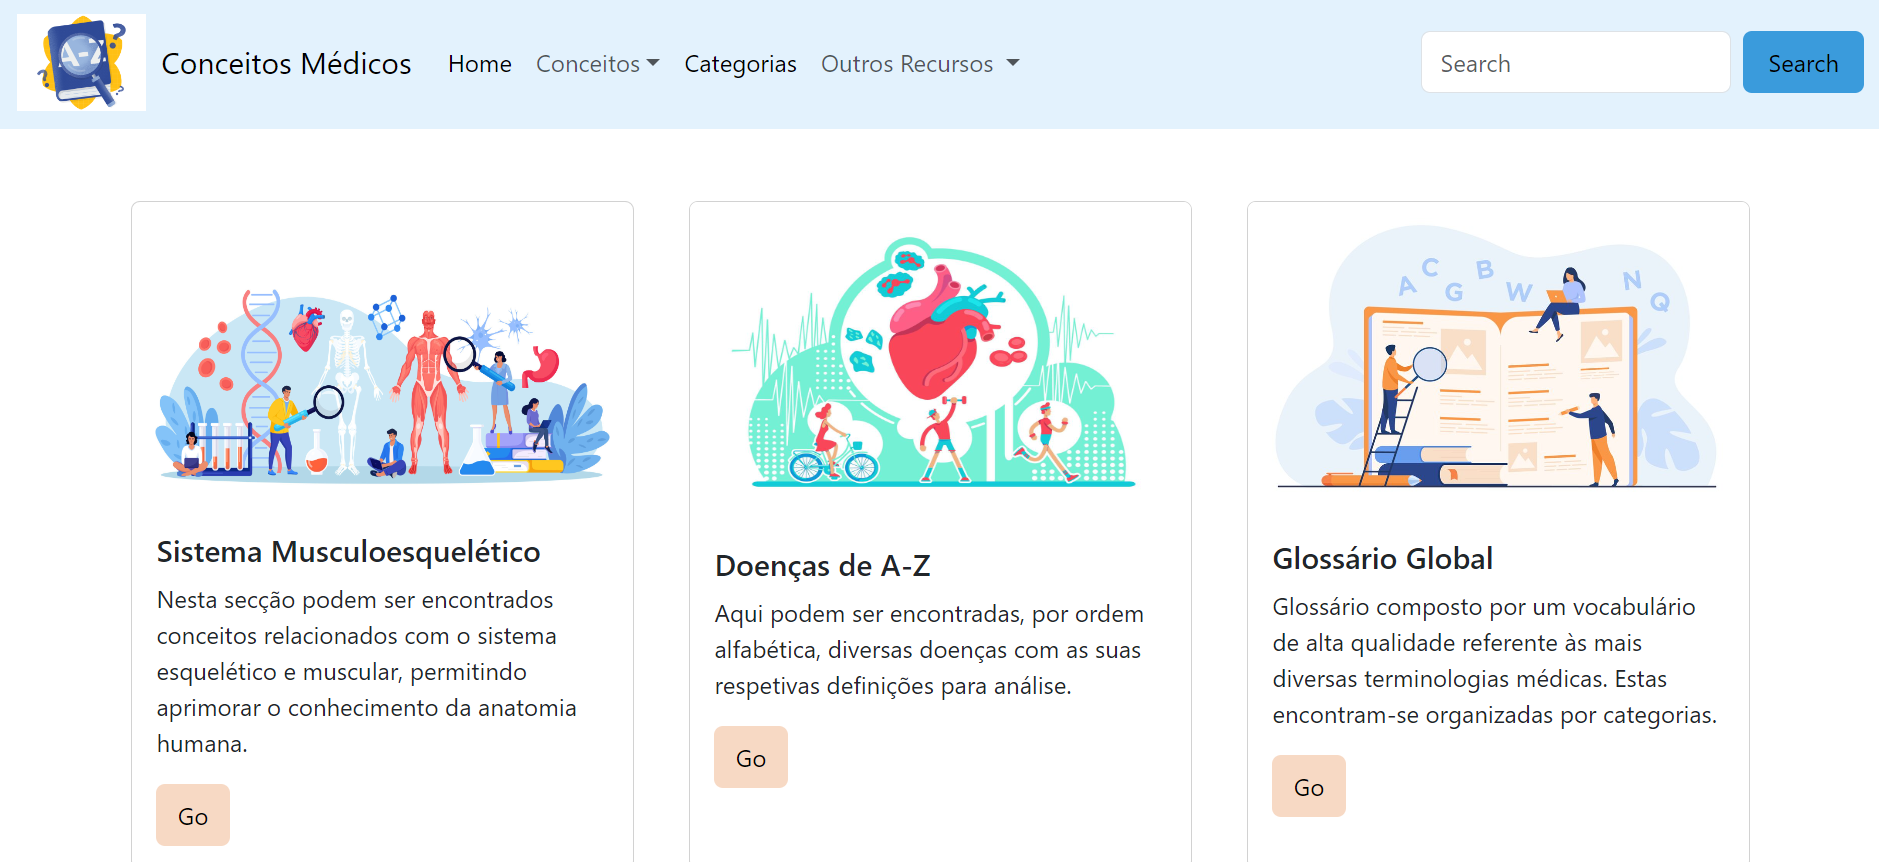
\includegraphics[width=0.9\textwidth]{Images/pag_inicial.png}
    \caption{Página Inicial}
    \label{fig:dic-traduc1}
\end{figure}

No que se refere à barra de navegação, podem ser encontradas as seguintes opções:

\begin{itemize}
    \item \textit{Home}, que, tal como o nome indica, redireciona o indivíduo para a página inicial da aplicação, ou seja, a página demonstrada na imagem anterior;

    \item \textit{Conceitos}, um menu suspenso, que, após a sua seleção, demonstra as opções "Sistema Musculoesquelético", "Doenças de A a Z" e "Glossário Global", pelo que cada uma permite transportar o utilizador para as respetivas páginas de listagem dos diversos conceitos;

    \begin{figure}[H]
        \centering
        \centering
        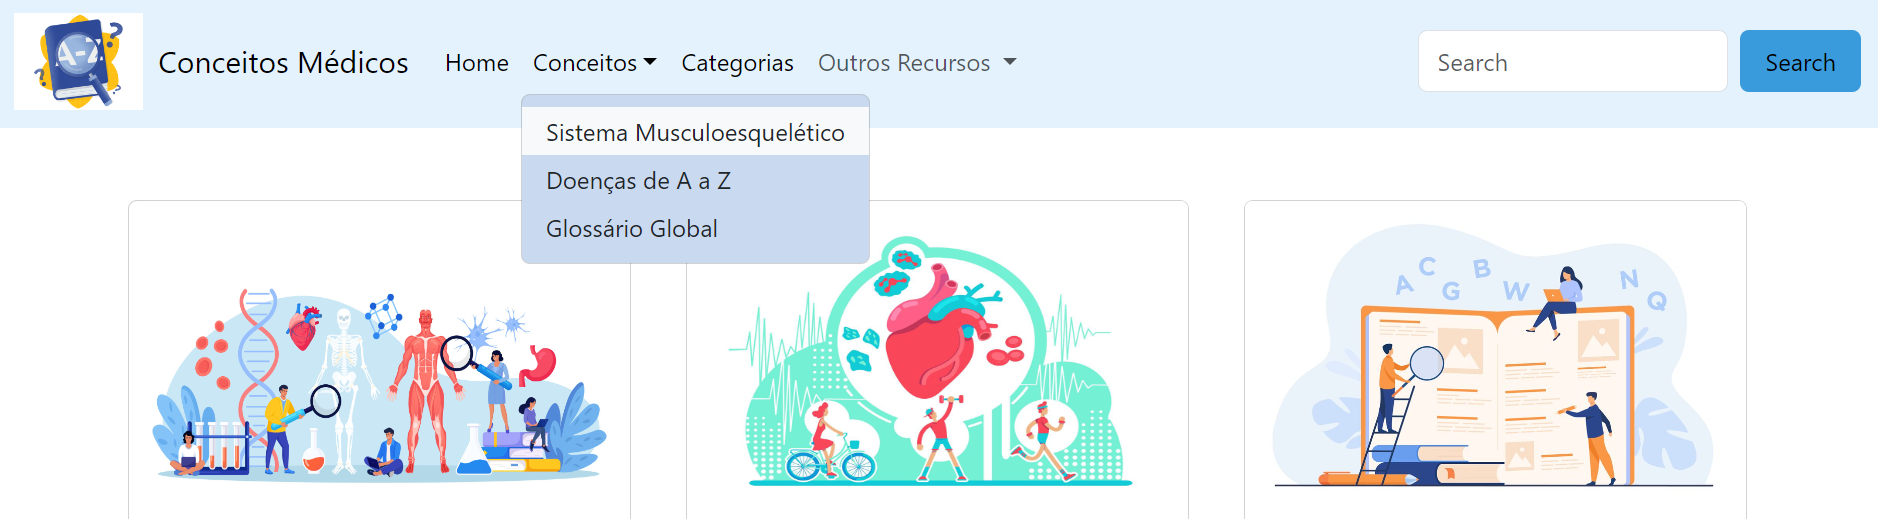
\includegraphics[width=0.9\textwidth]{Images/navbar_conceitos.png}
        \caption{Barra de navegação - Conceitos}
        \label{fig:dic-traduc1}
    \end{figure}

    \item \textit{Categorias}, que, tal como o nome indica, redireciona o indivíduo para uma página que lista todas as categorias dos termos em causa. Na imagem abaixo, é possível observar esta lista, pelo que, para facilitar o processo de procura, é disponibilizada uma filtragem por alfabeto. Por exemplo, após selecionar a letra "E", o utilizador é imediatamente transportado para a secção da lista onde começam as categorias inicializadas pela letra "E".

    \begin{figure}[H]
        \centering
        \centering
        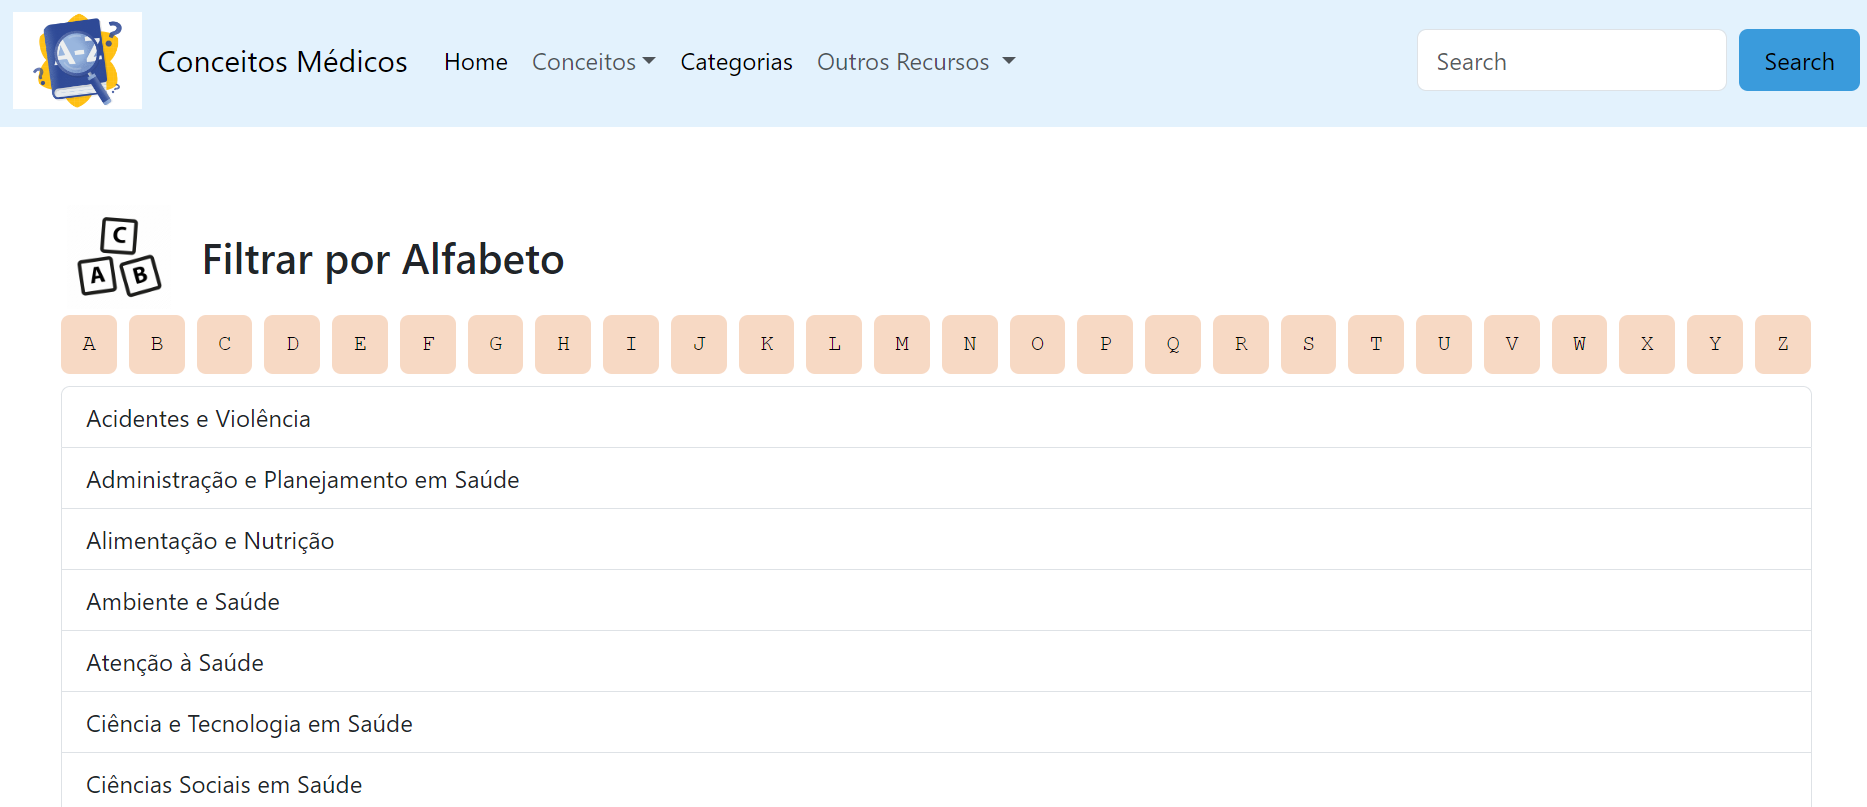
\includegraphics[width=0.9\textwidth]{Images/navbar_categorias.png}
        \caption{Listagem das Categorias}
        \label{fig:dic-traduc1}
    \end{figure}

    Neste caso, após a seleção da categoria "Atenção à Saúde", a página específica da mesma é exibida, juntamente com a disponibilização do botão "Ir para termos", que, tal como o nome indica, permite redirecionar o utilizador para página de listagem dos conceitos que pertencem a essa categoria.

    \begin{figure}[H]
        \centering
        \centering
        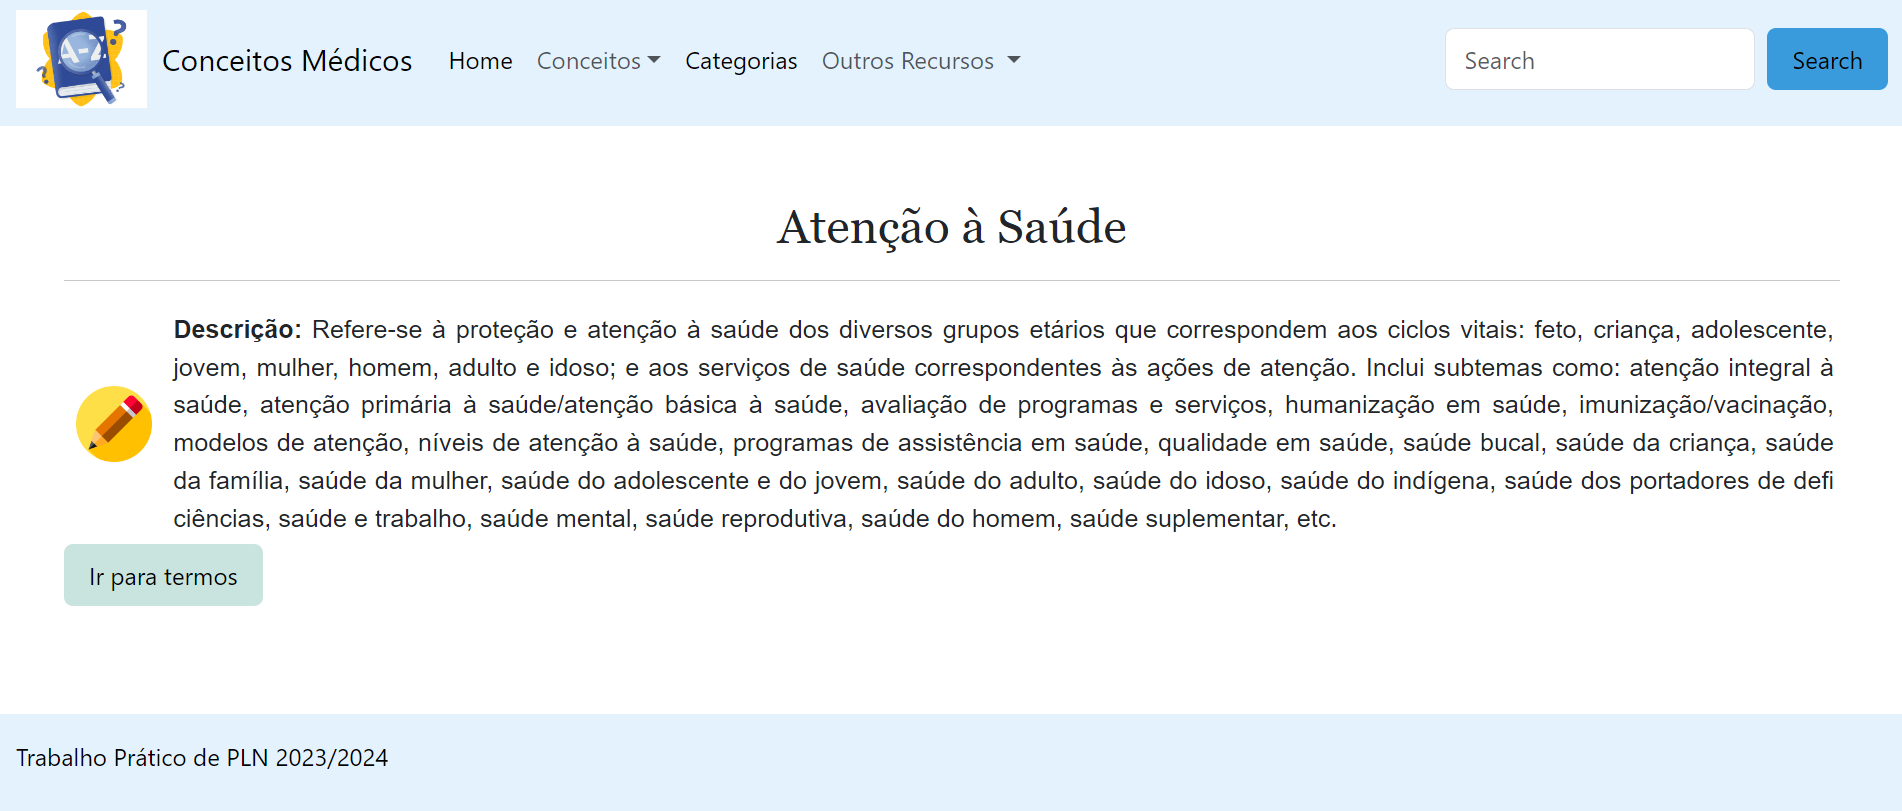
\includegraphics[width=0.9\textwidth]{Images/cat_especifica.png}
        \caption{Página específica de uma categoria}
        \label{fig:dic-traduc1}
    \end{figure}
    
    \item \textit{Outros Recursos}, um outro menu suspenso, que, neste caso, permite fornecer diferentes meios de auxílio ao utilizador, como, alguns dicionários médicos \textit{online}, ou, ainda, jogos que permitem colocar em prática o conhecimento acerca dos demais conceitos de saúde.
    Assim, na imagem abaixo, é possível averiguar que, após a seleção de "Outros Dicionários", um outro menu é exibido, sendo este composto por várias opções de dicionários médicos, como \textit{Harvard Medical School}, \textit{Merriam Webster} e \textit{Family Doctor}. Após a escolha de um destes, uma nova aba é aberta, sendo esta correspondente ao \textit{website} que contém o dicionário selecionado.

    \begin{figure}[H]
        \centering
        \centering
        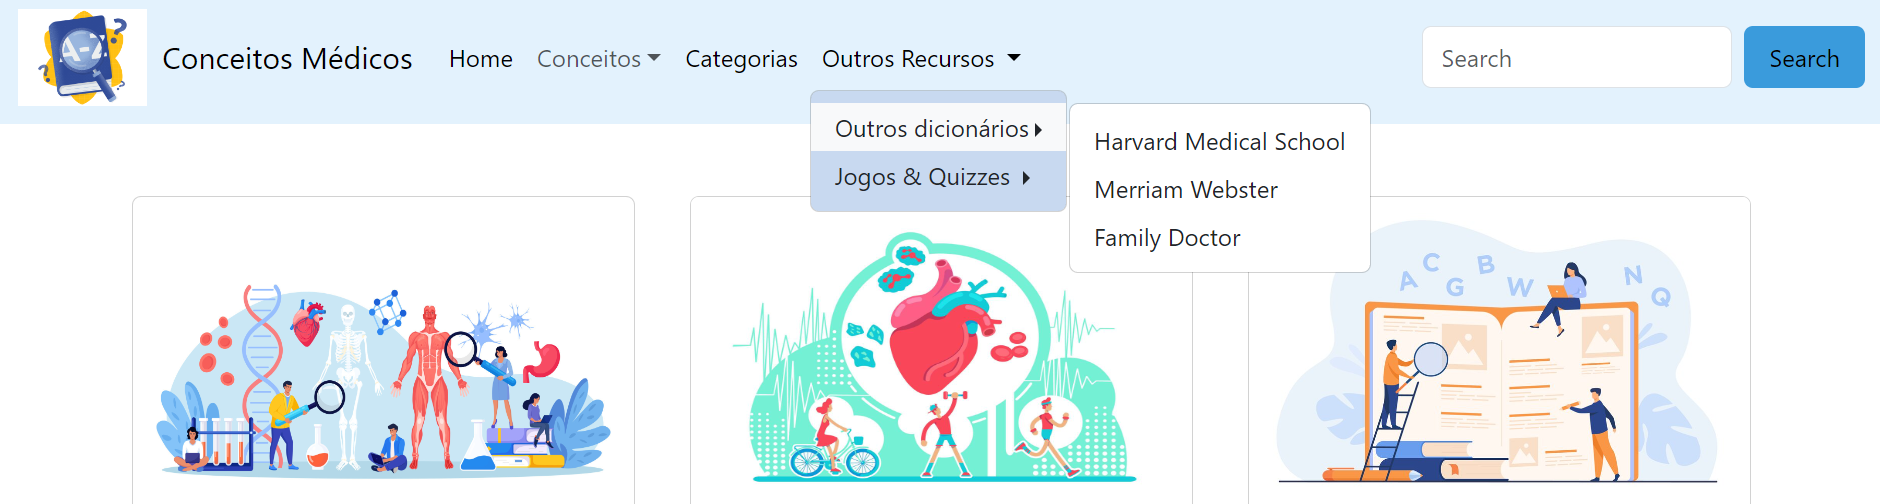
\includegraphics[width=0.9\textwidth]{Images/navbar_recursos.png}
        \caption{Barra de navegação - Outros Recursos}
        \label{fig:dic-traduc1}
    \end{figure}

    \item \textit{Search}, finalmente, surge a opção \textit{Search} que permite ao utilizador pesquisar por um determinado conceito. Aqui, é importante notar que a aplicação foi desenvolvida por forma a fornecer ao indivíduo toda a informação acerca do termo, podendo este estar presente em mais do que um conjunto de dados.\\
    A imagem abaixo permite demonstrar o resultado de pesquisa para "frontal", onde é possível denotar que esta palavra apenas se encontra presente em conceitos contidos no conjunto de dados relativo ao Sistema Musculoesquelético. Para além disso, qualquer ocorrência do termo pesquisado é destacada a amarelo, assim como qualquer um dos conceitos exibidos é sublinhado, para que o utilizador saiba que pode proceder à sua seleção por forma a ser redirecionado para a página específica do conceito.

    \begin{figure}[H]
        \centering
        \centering
        
\includegraphics[width=0.4\textwidth]{Images/pesquisa1.png}
        \caption{Barra de navegação - Search}
        \label{fig:dic-traduc1}
    \end{figure}

    \begin{figure}[H]
        \centering
        \centering
        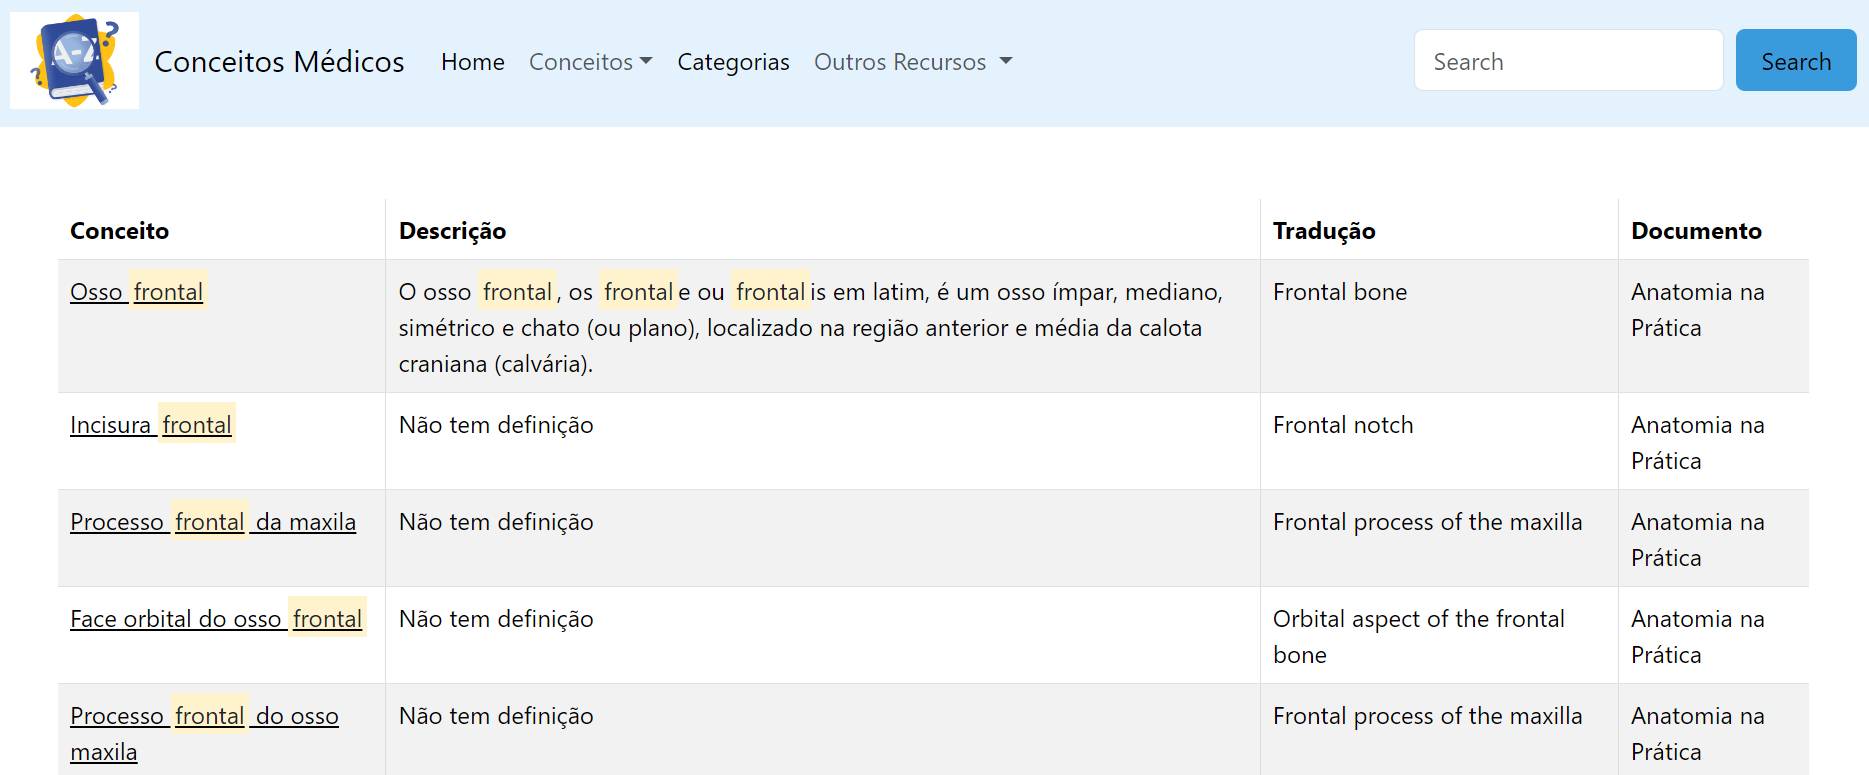
\includegraphics[width=0.9\textwidth]{Images/pesquisa2.png}
        \caption{Resultados da pesquisa para "frontal"}
        \label{fig:dic-traduc1}
    \end{figure}

    Todavia, caso a palavra pesquisada pelo utilizador não se encontre presente em nenhum dos conjuntos de dados, um \textit{template} HTML de erro é renderizado de maneira a dar a conhecer ao indivíduo que o termo não foi encontrado. Quando esta situação acontece, é disponibilizado um botão que permite retornar à página inicial da aplicação.

    \begin{figure}[H]
        \centering
        \centering
        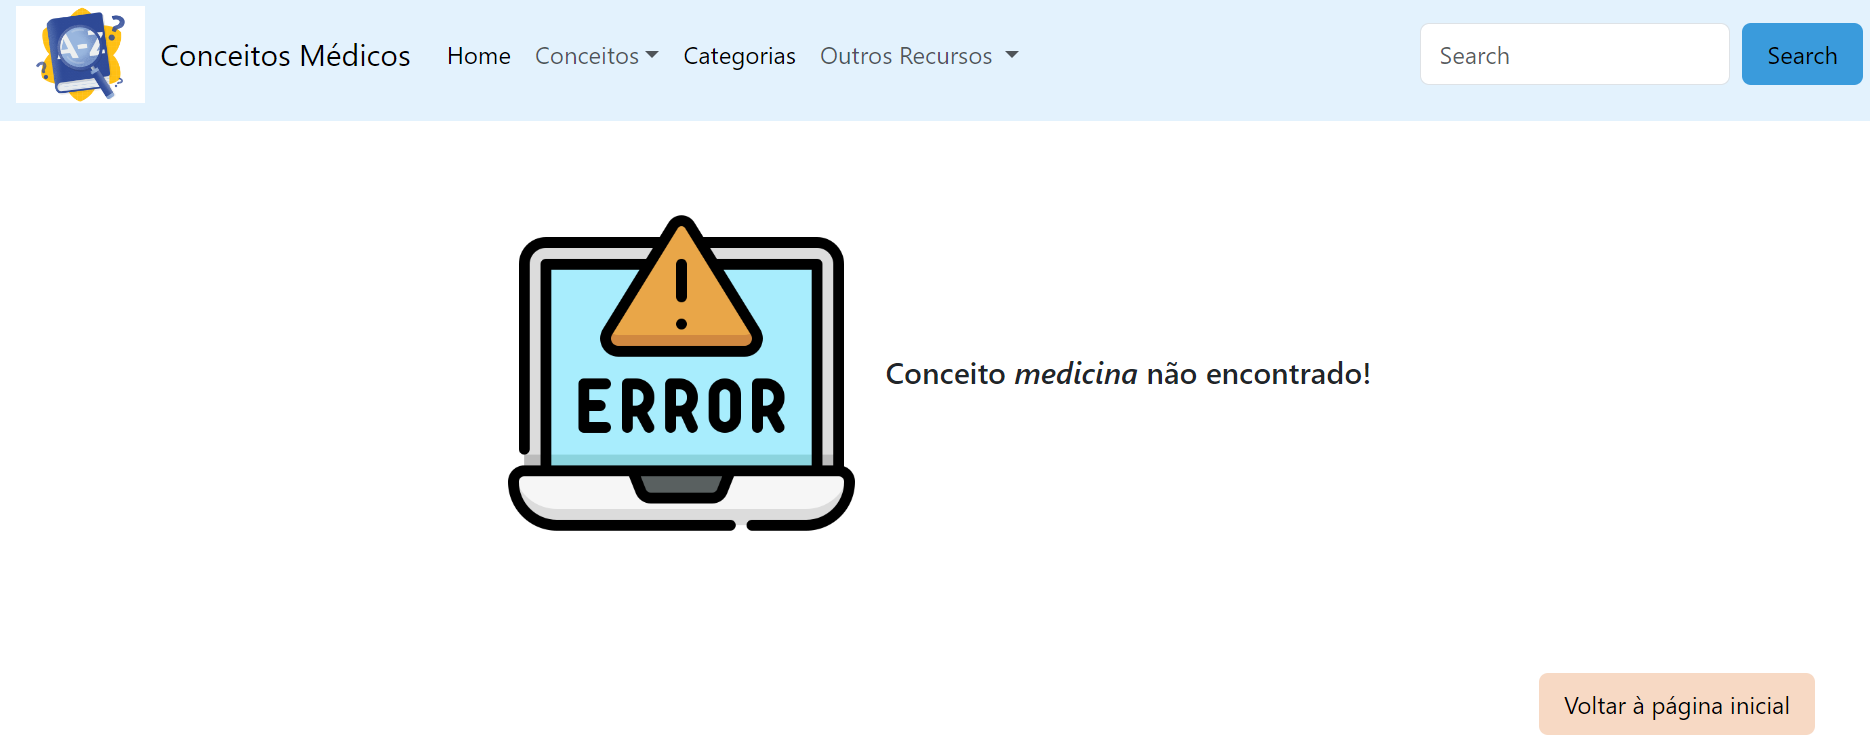
\includegraphics[width=0.9\textwidth]{Images/pesquisa3.png}
        \caption{Resultados da pesquisa para "medicina"}
        \label{fig:dic-traduc1}
    \end{figure}
    
\end{itemize}

\subsection{Plataforma Web - Funcionalidades}

\subsubsection{Sistema Musculoesquelético}

Tal como foi referido na secção relativa à página inicial, após o utilizador clicar no botão \textit{Go}, presente no bloco relativo ao Sistema Musculoesquelético, o mesmo é redirecionado para a página de listagem dos demais conceitos pertencentes a esse conjunto de dados.

\textbf{Filtragem por Categorias:}\\

Uma parte inicial dessa página pode ser averiguada na imagem abaixo, onde o indivíduo se depara com a possibilidade de filtrar os conceitos pelas várias categorias existentes, quer para o Sistema Esquelético e Articular, quer para o Sistema Muscular.

\begin{figure}[H]
    \centering
    \centering
    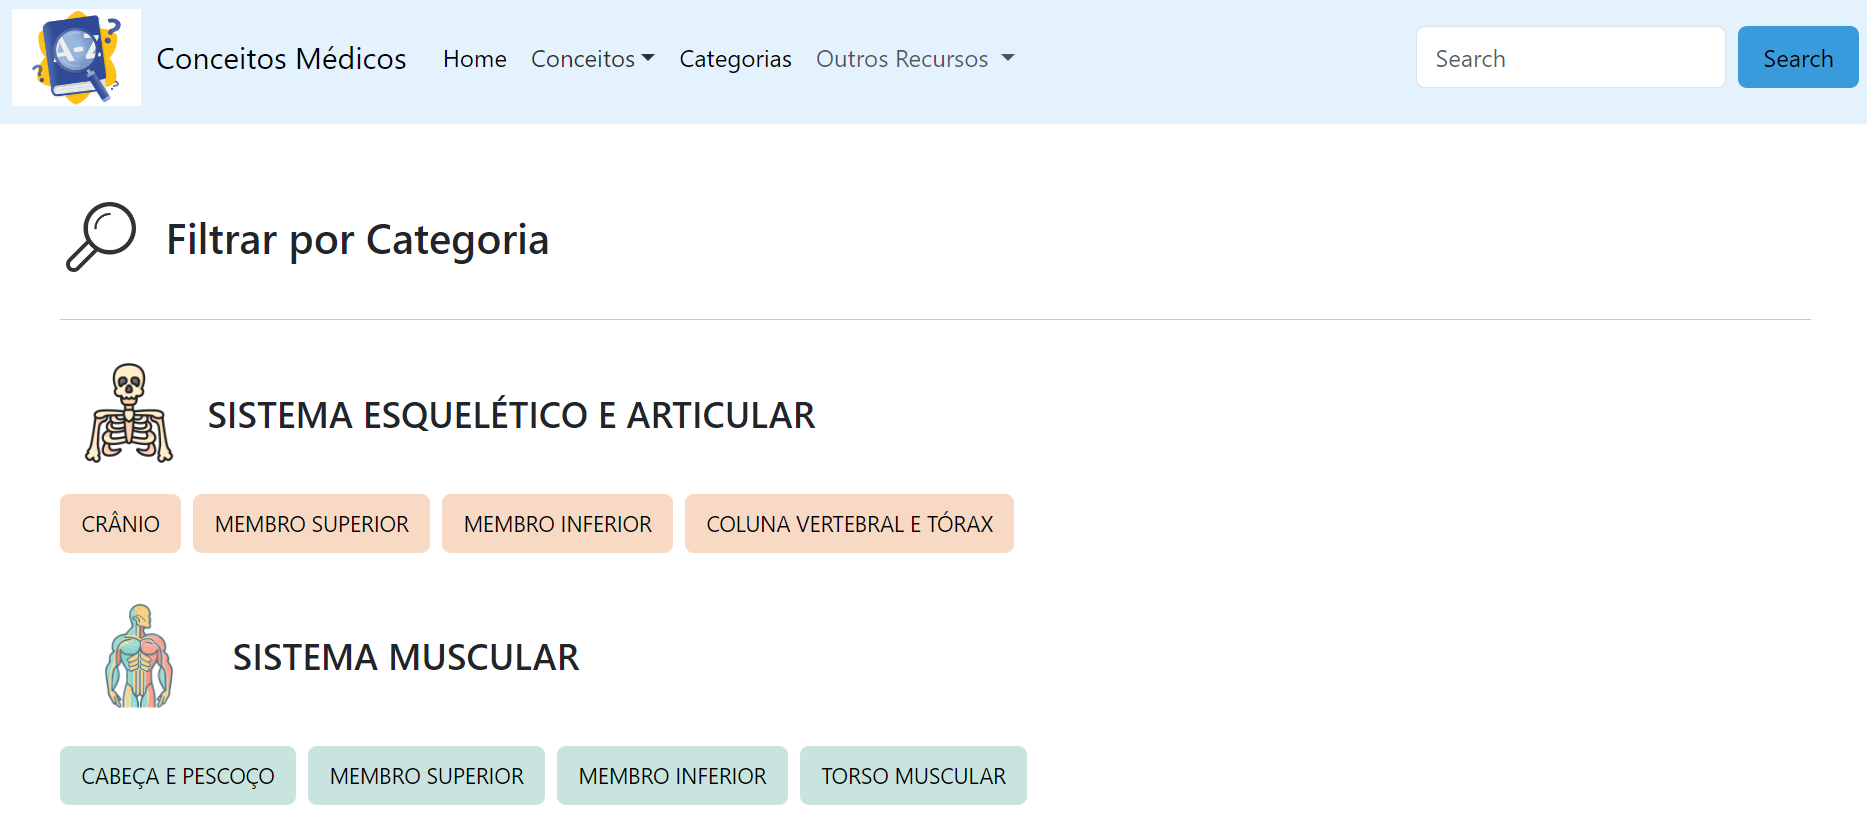
\includegraphics[width=0.9\textwidth]{Images/musculo1.png}
    \caption{Página Inicial do Sistema Musculoesquelético}
    \label{fig:dic-traduc1}
\end{figure}

A título de exemplo, depois de ser selecionada a categoria "Membro Superior", do Sistema Esquelético e Articular, o utilizador é imediatamente redirecionado para o conjunto de conceitos pertencentes a esse grupo.

\textbf{Adicionar novo conceito:}\\

Adicionalmente, ainda na página inicial relativa ao Sistema Musculoesquelético, após a filtragem por categorias, o utilizador tem, ainda, a possibilidade de adicionar um novo conceito, ao conjunto de dados, após clicar no sinal de \+.

Quando isto se verifica, uma nova janela, de menor dimensão, é aberta para que possam ser introduzidas as informações descritivas do termo a adicionar.

\begin{figure}[H]
    \centering
    \centering
    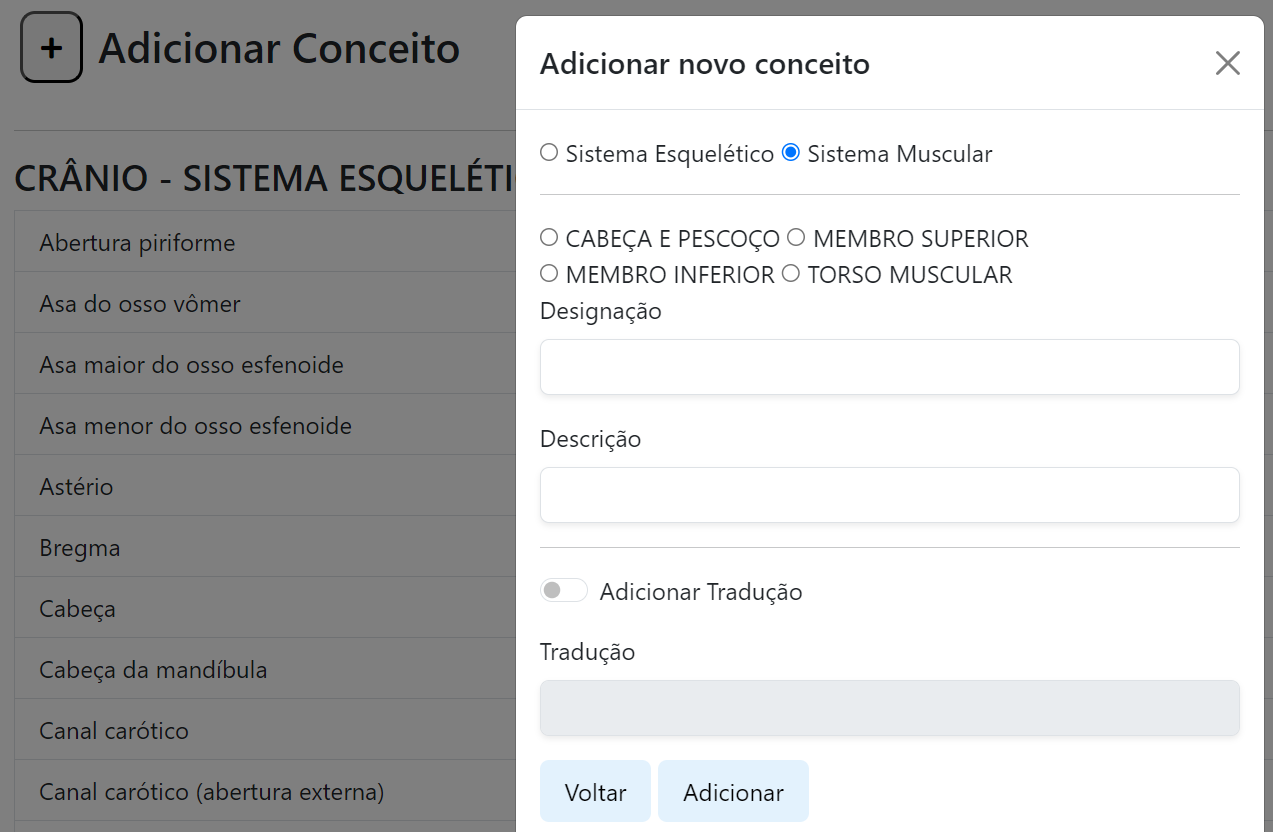
\includegraphics[width=0.7\textwidth]{Images/musculo_adicionar.png}
    \caption{Adição de novo conceito - Sistema Musculoesquelético}
    \label{fig:dic-traduc1}
\end{figure}

Tal como é possível observar na figura acima, dois \textit{radio buttons} são disponibilizados para que o utilizador possa decidir o sistema a que o novo conceito pertence, isto é, ao Sistema Esquelético ou ao Sistema Muscular. Após efetuar a sua escolha, um novo conjunto de \textit{radio buttons} é exibido, tratando-se estes das várias categorias, específicas do sistema selecionado. Este comportamento foi conseguido graças ao estabelecimento de um \textit{JavaScript} que faz com os restantes \textit{radio buttons} surjam, apenas quando o utilizador seleciona um dos dois botões disponibilizados inicialmente.

Depois de ser selecionada uma determinada categoria, o indivíduo pode, então, proceder ao preenchimento dos campos "Designação", "Descrição" e "Tradução". É importante notar que esta última não é de preenchimento obrigatório, podendo o indivíduo, ativar, ou desativar, o campo de preenchimento.
Finalmente, dois botões são disponibilizados, isto é, um botão "Voltar" que retorna à página de listagem de conceitos e um botão "Adicionar", que, tal como o nome indica, adiciona o novo conceito ao ficheiro JSON.

\begin{figure}[H]
    \centering
    \centering
    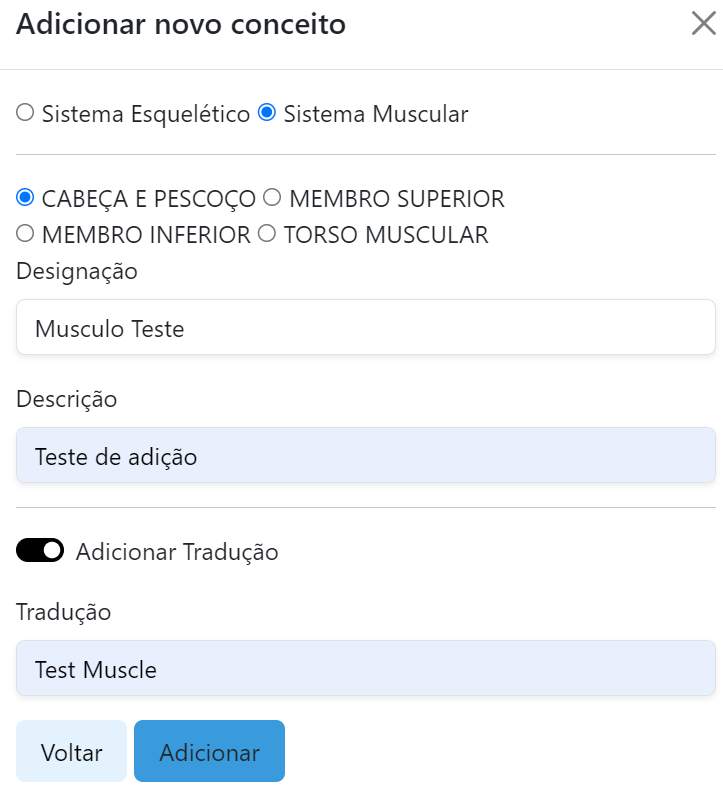
\includegraphics[width=0.5\textwidth]{Images/add_ex.png}
    \caption{Adição de novo conceito - Sistema Musculoesquelético, exemplo}
    \label{fig:dic-traduc1}
\end{figure}

\begin{figure}[H]
    \centering
    \centering
    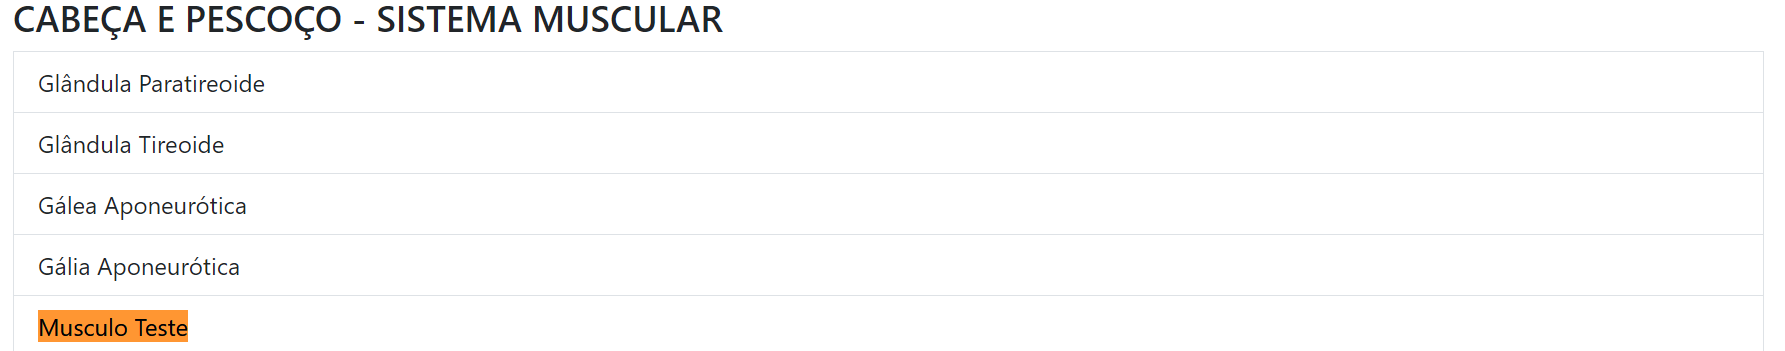
\includegraphics[width=0.9\textwidth]{Images/add_ex2.png}
    \caption{Resultado da adição de novo conceito - Sistema Musculoesquelético}
    \label{fig:dic-traduc1}
\end{figure}

As duas figuras acima exemplificam o processo de adição de um novo conceito, neste caso, o conceito com designação "Musculo Teste". É de capital importância referir que se procedeu à garantia de um \textit{backup}, para que, caso a aplicação fosse reiniciada, o conceito adicionado permanecesse no conjunto de dados. Tal foi conseguido pela abertura do ficheiro JSON para posterior escrita do novo dicionário atualizado. Adicionalmente, apenas se procede à adição do novo termo, se os demais campos não se encontrarem vazios e se a designação do mesmo não existir para a categoria em causa.

\textbf{Editar Descrição \& Adicionar Tradução de um conceito:}\\

Partindo do conceito anteriormente adicionado, isto é, o conceito cuja designação corresponde a "Musculo Teste", a sua seleção, na lista composta por todos os conceitos, redireciona o utilizador para a página específica do termo, que pode ser analisada na imagem que se segue:

\begin{figure}[H]
    \centering
    \centering
    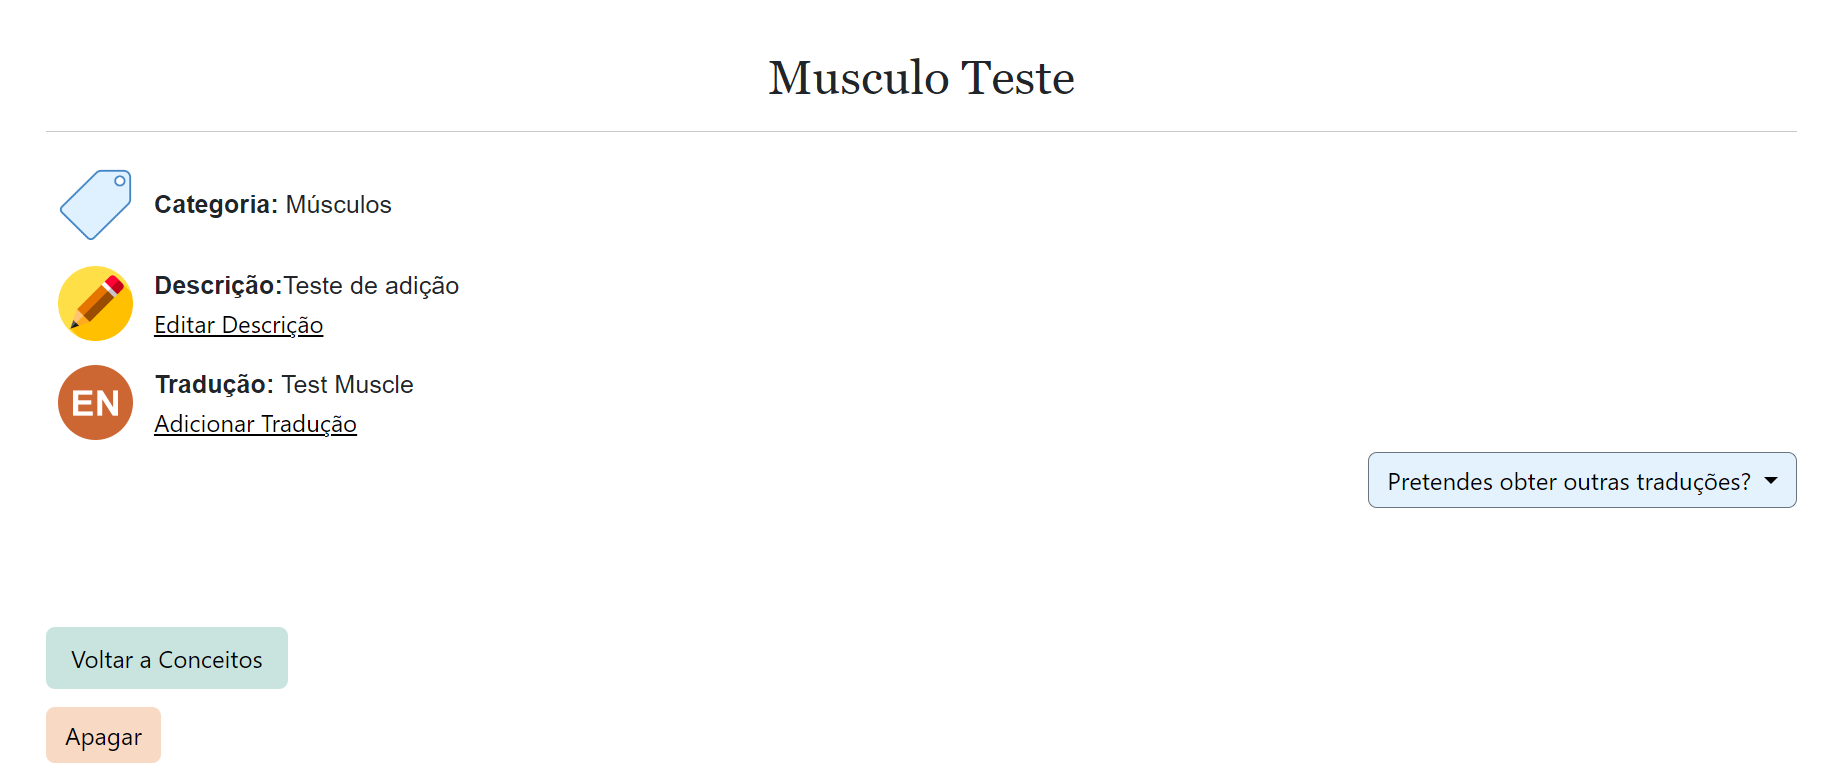
\includegraphics[width=0.9\textwidth]{Images/termo1.png}
    \caption{Página específica do conceito - Sistema Musculoesquelético}
    \label{fig:dic-traduc1}
\end{figure}

Aqui, encontram-se, como parâmetros descritivos do termo, a categoria a que pertence, a sua descrição e a sua tradução. No que se refere a estes dois últimos, é de notar a presença das opções "Editar Descrição" e "Adicionar Tradução", respetivamente.

Relativamente à primeira opção, após a sua seleção, uma nova página é exibida, com um campo de preenchimento da nova descrição.

\begin{figure}[H]
    \centering
    \centering
    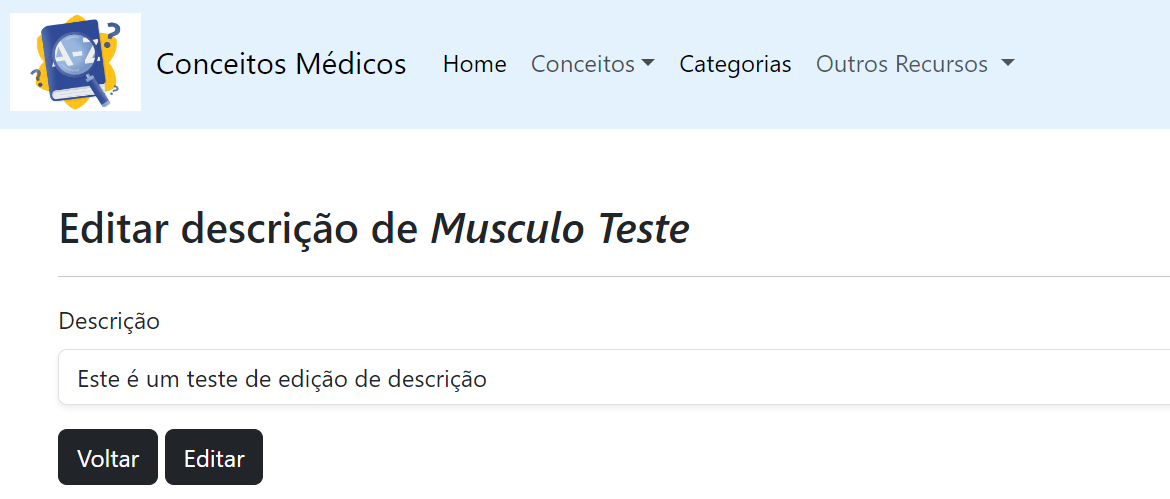
\includegraphics[width=0.7\textwidth]{Images/termo_editar_desc.png}
    \caption{Edição de descrição do conceito - Sistema Musculoesquelético}
    \label{fig:dic-traduc1}
\end{figure}

Na imagem acima, procedeu-se à alteração da descrição original para "Este é um teste de edição de descrição", pelo que, a seleção do botão "Editar" torna a operação efetiva, enquanto que o botão "Voltar" descarta essa alteração.

A figura abaixo trata-se de um caso em que a alteração, foi, efetivamente, implementada, dado que se pode observar a nova descrição introduzida.

\begin{figure}[H]
    \centering
    \centering
    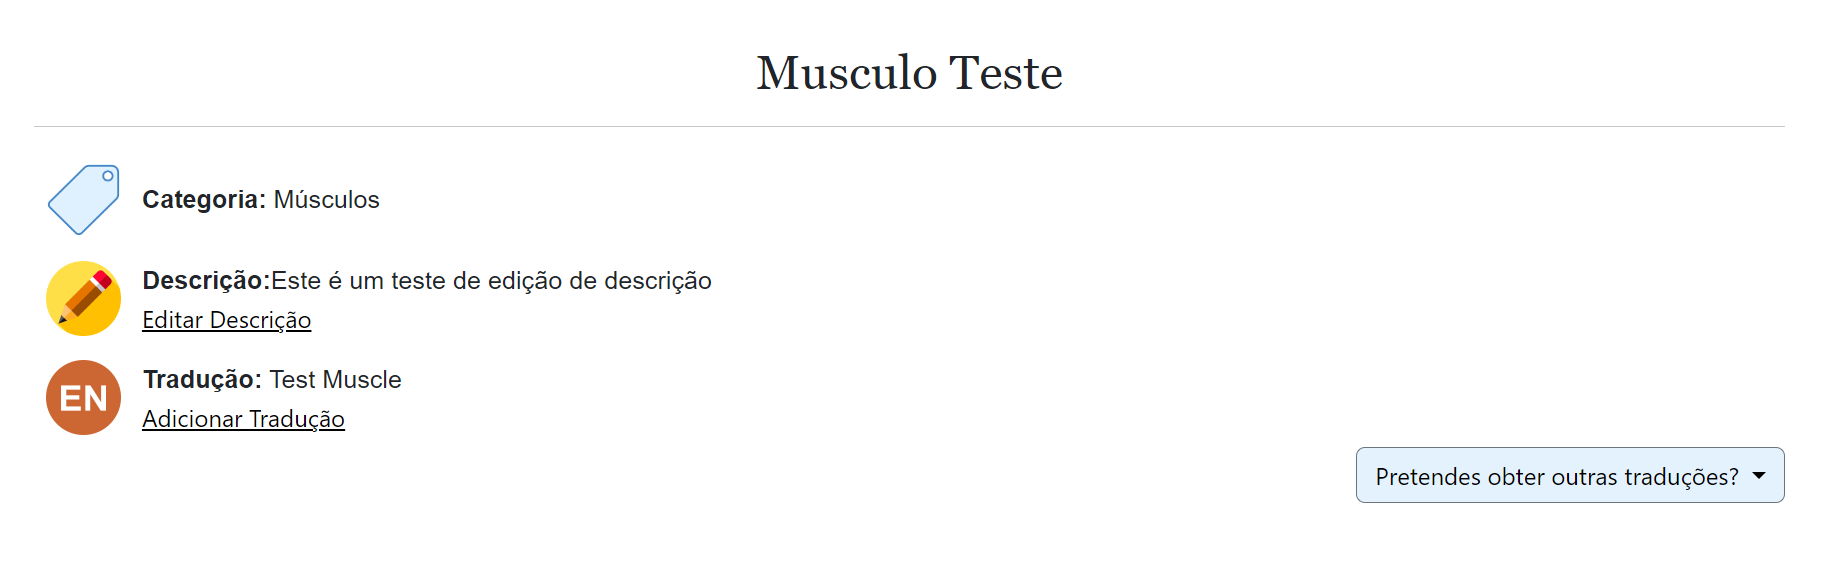
\includegraphics[width=0.9\textwidth]{Images/termo_desc_editada.png}
    \caption{Edição de descrição do conceito - Sistema Musculoesquelético}
    \label{fig:dic-traduc1}
\end{figure}

Relativamente à operação de "Adicionar Tradução", de igual modo, é exibida uma nova página, para que o indivíduo possa proceder à concretização da alteração.

\begin{figure}[H]
    \centering
    \centering
    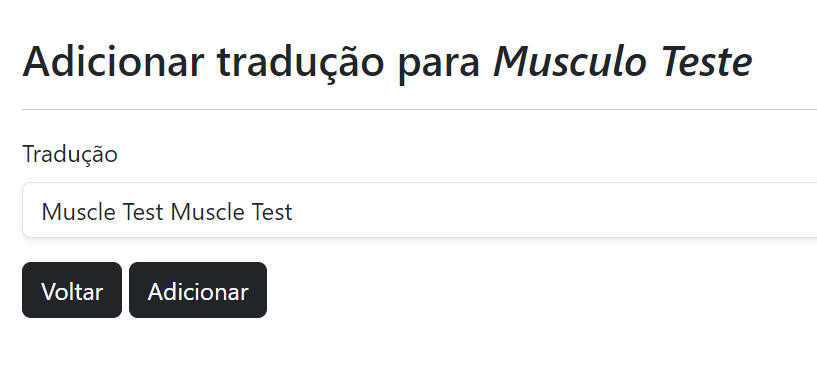
\includegraphics[width=0.6\textwidth]{Images/termo_add_trad.png}
    \caption{Adicionar Tradução a conceito - Sistema Musculoesquelético}
    \label{fig:dic-traduc1}
\end{figure}

Neste caso, o botão "Adicionar" torna a alteração efetiva, enquanto que o botão "Voltar" descarta essa alteração.

A figura abaixo trata-se de um caso em que a alteração, foi, efetivamente, implementada, dado que se pode observar a nova tradução introduzida.

\begin{figure}[H]
    \centering
    \centering
    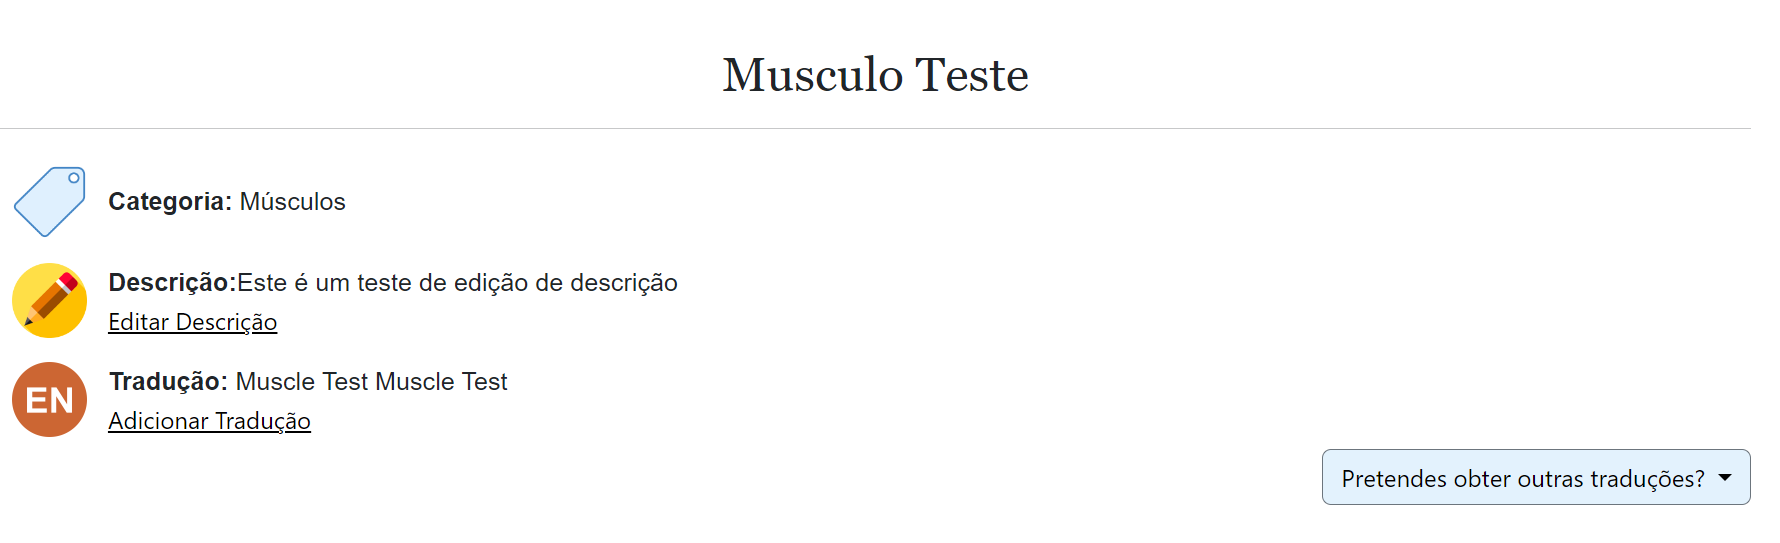
\includegraphics[width=0.9\textwidth]{Images/termo_desc_trad_editada.png}
    \caption{Adição de Tradução e Edição de descrição a conceito - Sistema Musculoesquelético}
    \label{fig:dic-traduc1}
\end{figure}

Tal como na funcionalidade anterior, procedeu-se, de igual modo, à garantia de um \textit{backup}, para que, caso a aplicação fosse reiniciada, as novas alterações permanecessem no conjunto de dados. Tal foi conseguido pela abertura do ficheiro JSON para posterior escrita do novo dicionário atualizado.


\textbf{Eliminação de um conceito:}\\

Na página específica de um determinado conceito é possível averiguar a presença de um botão com a descrição "Apagar". Tal como o nome indica, o mesmo tem como principal objetivo eliminar o conceito em causa do conjunto de dados.

Caso este seja selecionado, uma janela \textit{pop-up} é aberta de maneira a questionar ao utilizador se pretende mesmo descartar o termo em questão. Caso o indivíduo selecione "Voltar", o mesmo é retornado para a página do conceito, caso contrário, a seleção do botão "Apagar" efetua a operação em causa.

\begin{figure}[H]
    \centering
    \centering
    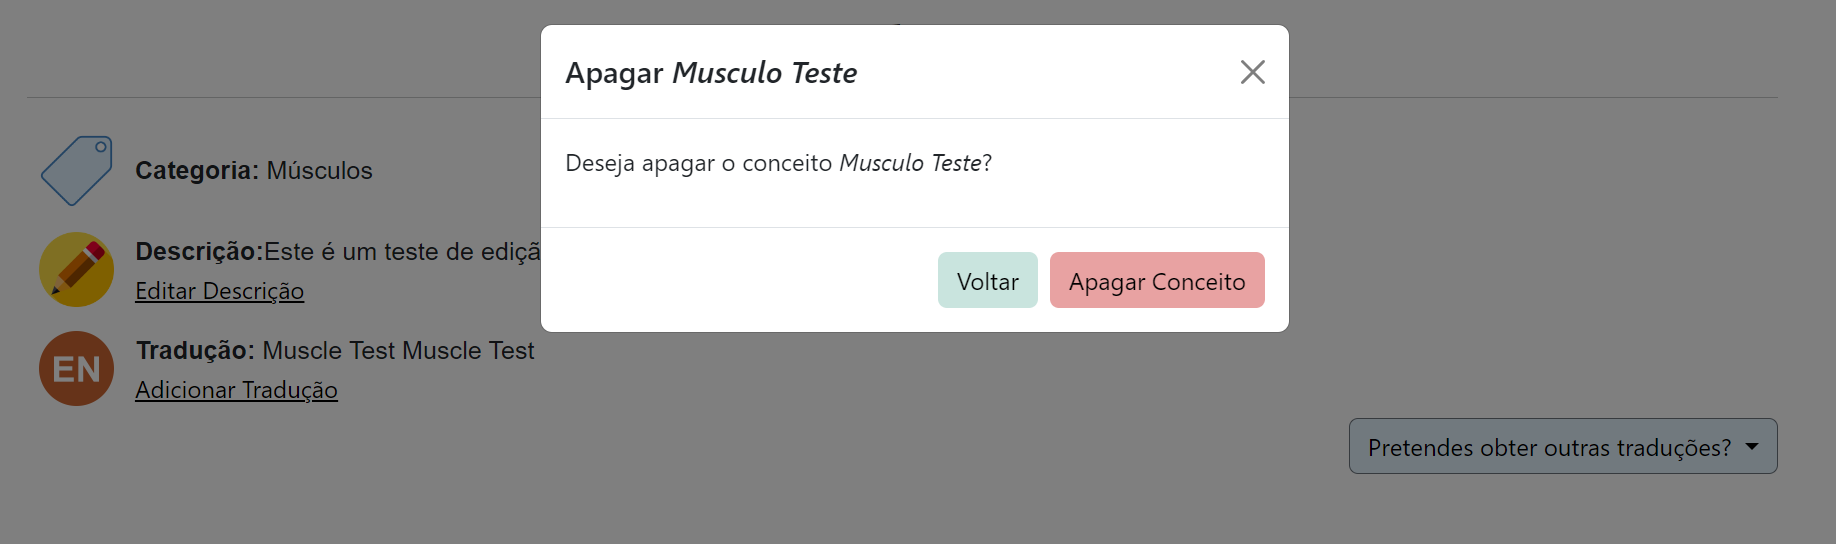
\includegraphics[width=0.9\textwidth]{Images/apagar_termo.png}
    \caption{Eliminação de um conceito - Sistema Musculoesquelético}
    \label{fig:dic-traduc1}
\end{figure}

De maneira a garantir a persistência das novas alterações, foi estabelecido um \textit{backup}, através da eliminação inicial do conceito do dicionário (pelo método \textit{del}) e posterior escrita, do dicionário atualizado, no ficheiro JSON.

\textbf{Obtenção de novas traduções do conceito:}\\

A figura abaixo refere-se à página específica para o termo \textit{Canal Carótico}, onde é possível constatar a presença de um botão, com a descrição "Pretendes obter outras traduções?".
Este componente, após a sua seleção, permite exibir um menu suspenso, composto por várias línguas tais como Espanhol, Francês, Italiano e Alemão, para que, após a escolha de um determinado idioma, o utilizador seja redirecionado diretamente para o \textit{Google Tradutor}, que exibe, imediatamente, a tradução desejada.

\begin{figure}[H]
    \centering
    \centering
    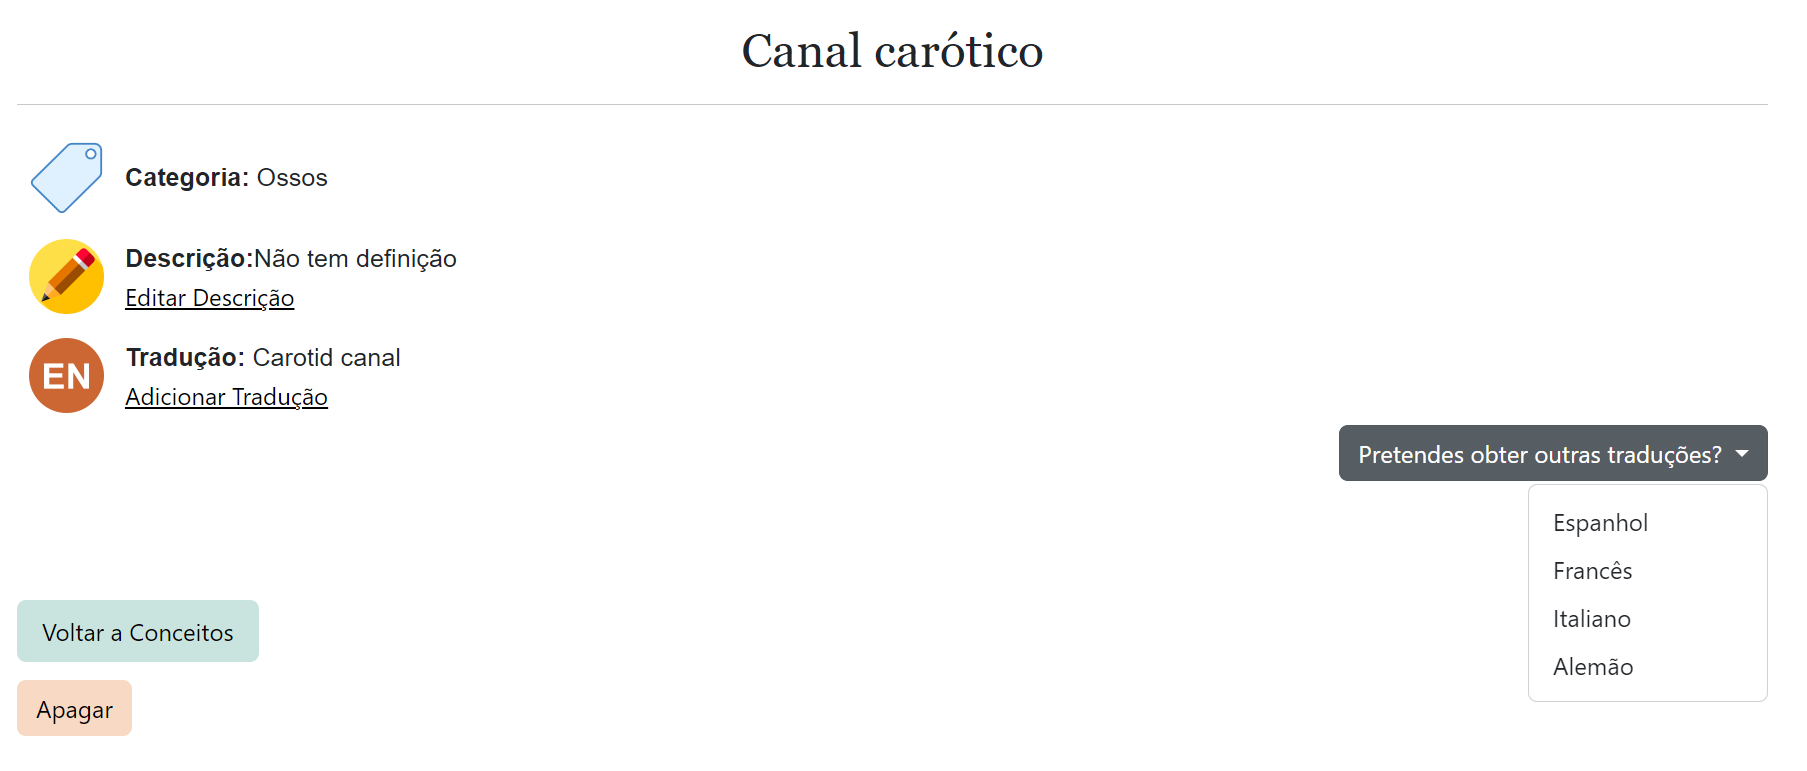
\includegraphics[width=0.9\textwidth]{Images/outras_trad.png}
    \caption{Obtenção de novas traduções - Sistema Musculoesquelético}
    \label{fig:dic-traduc1}
\end{figure}

\begin{figure}[H]
    \centering
    \centering
    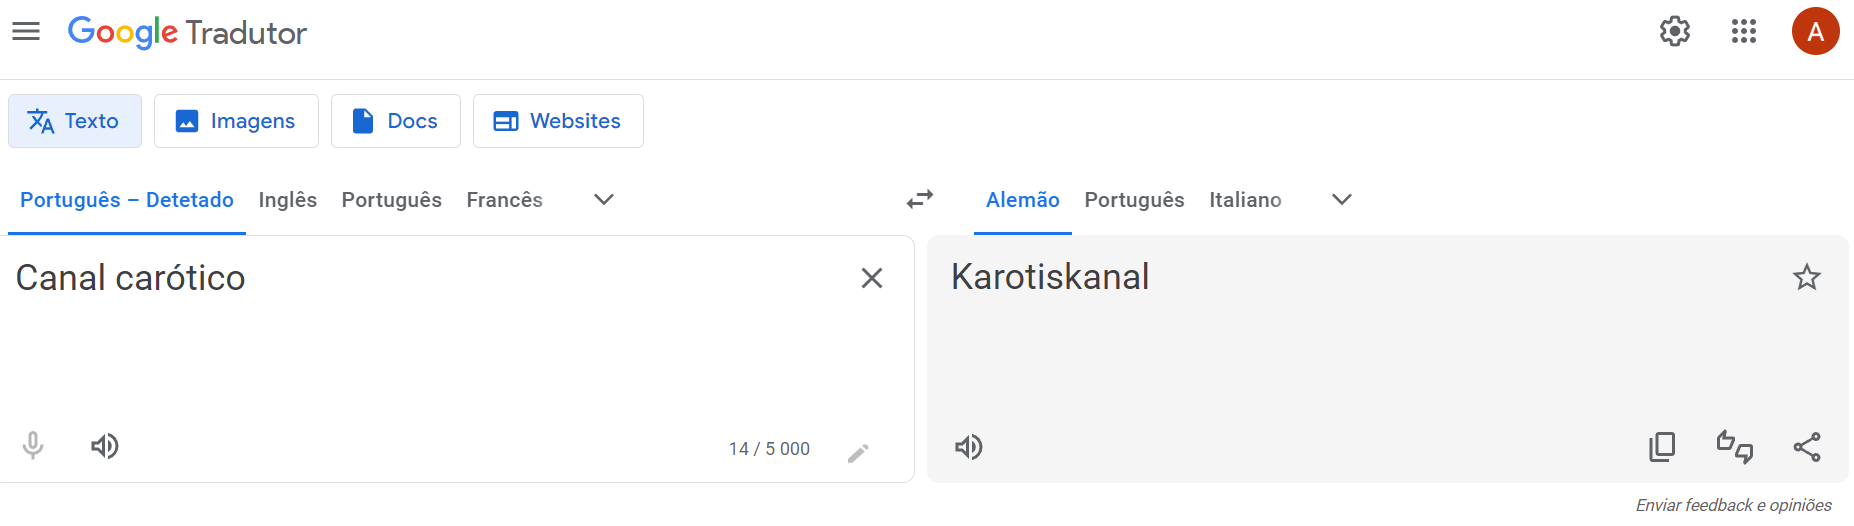
\includegraphics[width=0.9\textwidth]{Images/tradutor.png}
    \caption{Obtenção de nova tradução - Sistema Musculoesquelético}
    \label{fig:dic-traduc1}
\end{figure}

Neste caso, a figura acima refere-se à situação em que foi selecionado como idioma o Alemão, pelo que uma nova janela foi aberta, com o resultado da tradução.

\subsubsection{Doenças de A-Z}

De maneira semelhante ao que foi descrito na secção anterior, é possível aceder à página com as designações das diferentes doenças através do botão \textit{Go}, presente no bloco "Doenças de A-Z".

Nesta página inicial, é possível verificar, por ordem alfabética, todas as enfermidades presentes na plataforma, bem como, através dos botões referentes às letras, mover-se diretamente para a porção da página com os conceitos que começam com a letra selecionada.

\begin{figure}[H]
    \centering
    \centering
    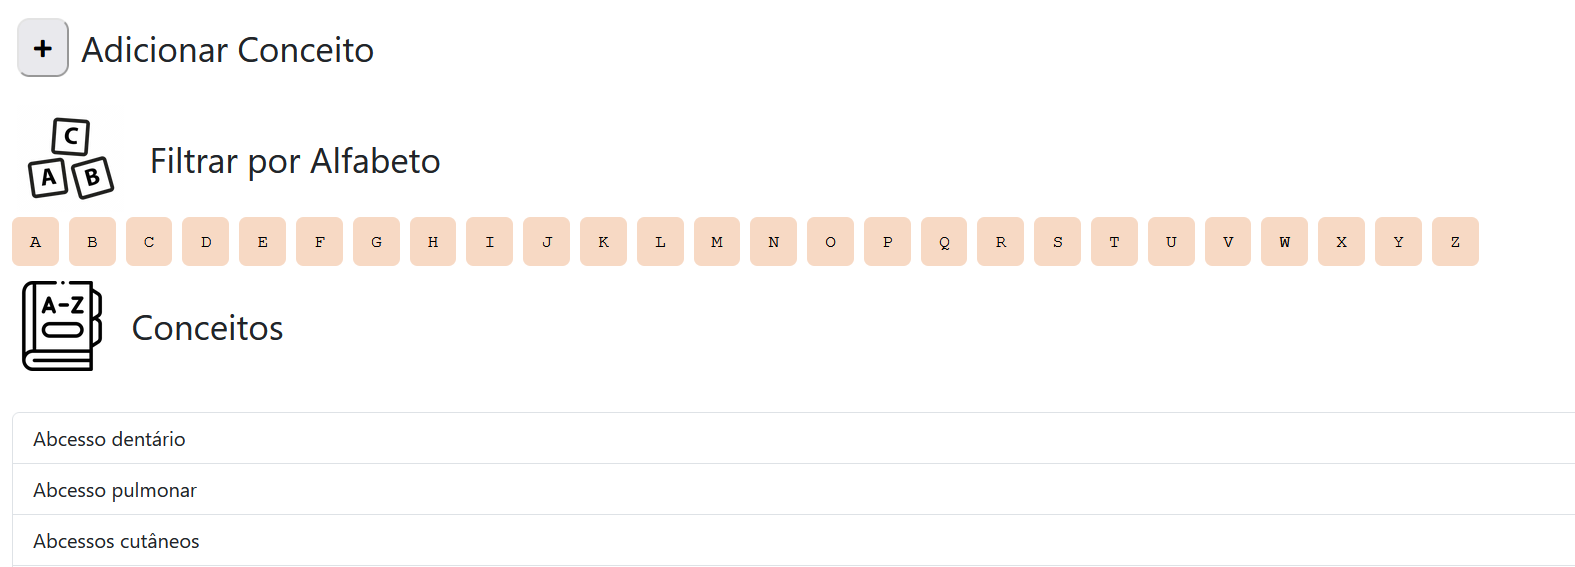
\includegraphics[width=0.9\textwidth]{Images/doencas_pag_inicial.png}
    \caption{Página inicial da secção Doenças de A-Z}
    \label{fig:dic-traduc1}
\end{figure}

\textbf{Adicionar novo conceito:}\\

No que se refere à adição de uma nova doença, esta pode ser feita a partir do botão "Adicionar conceito", presente na página inicial. Este botão abre uma janela sobreposta à página, na qual é possível adicionar a informação acerca do novo conceito. 

\begin{figure}[H]
    \centering
    \centering
    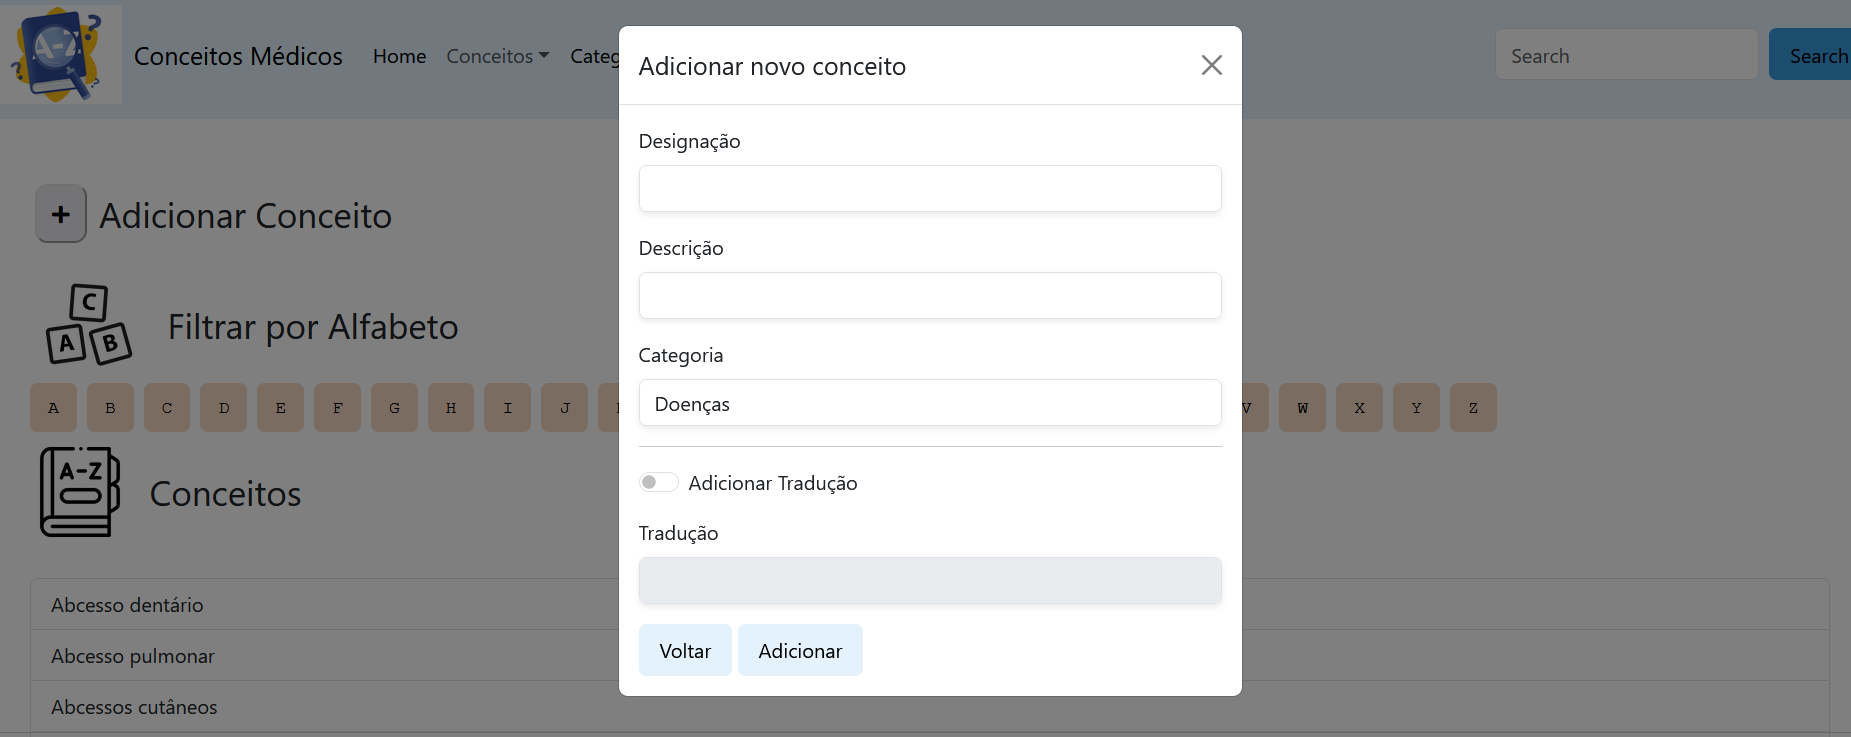
\includegraphics[width=0.9\textwidth]{Images/doencas_adicionar_conceito.png}
    \caption{Página inicial da secção Doenças de A-Z}
    \label{fig:dic-traduc1}
\end{figure}

Como podemos ver na imagem acima, o utilizador tem a oportunidade de adicionar a designação da nova doença, bem como a sua descrição, à semelhança do que acontece para a adição de novos elementos do Sistema Musculoesquelético. Pelo contrário, o parâmetro de categoria é preenchido automaticamente com "Doenças", não sendo permitida a sua alteração. 

Para além disso, o utilizador é capaz de decidir se deseja adicionar uma tradução da designação em inglês, utilizando o \textit{toggle button}. A ativação deste botão disponibiliza o elemento de \textit{input}, no qual o utilizador pode escrever a tradução desejada. 

Por fim, o utilizador pode adicionar o novo conceito ao \textit{site}, utilizando o botão "Adicionar", ou pode descartar a informação, utilizando o botão "Voltar," que o retorna para a página de conceitos.

\subsubsection{Glossário Global}

Assim como descrito nas secções anteriores, o botão \textit{Go} presente no bloco "Glossário Global" permite que o utilizador aceda à página com os diferentes conceitos relacionados à área da saúde.

Nesta página, é possível visualizar todos os termos ordenados alfabeticamente e um botão que permite adicionar um novo conceito. Além disso, como referido anteriormente, os conceitos presentes no glossário são classificados em categorias, portanto, foi adicionada à opção "Filtrar por categoria" que permite o utilizador especificar, através de um \textit{dropdown menu}, a categoria desejada para visualizar os conceitos correspondentes.

\begin{figure}[H]
    \centering
    \centering
    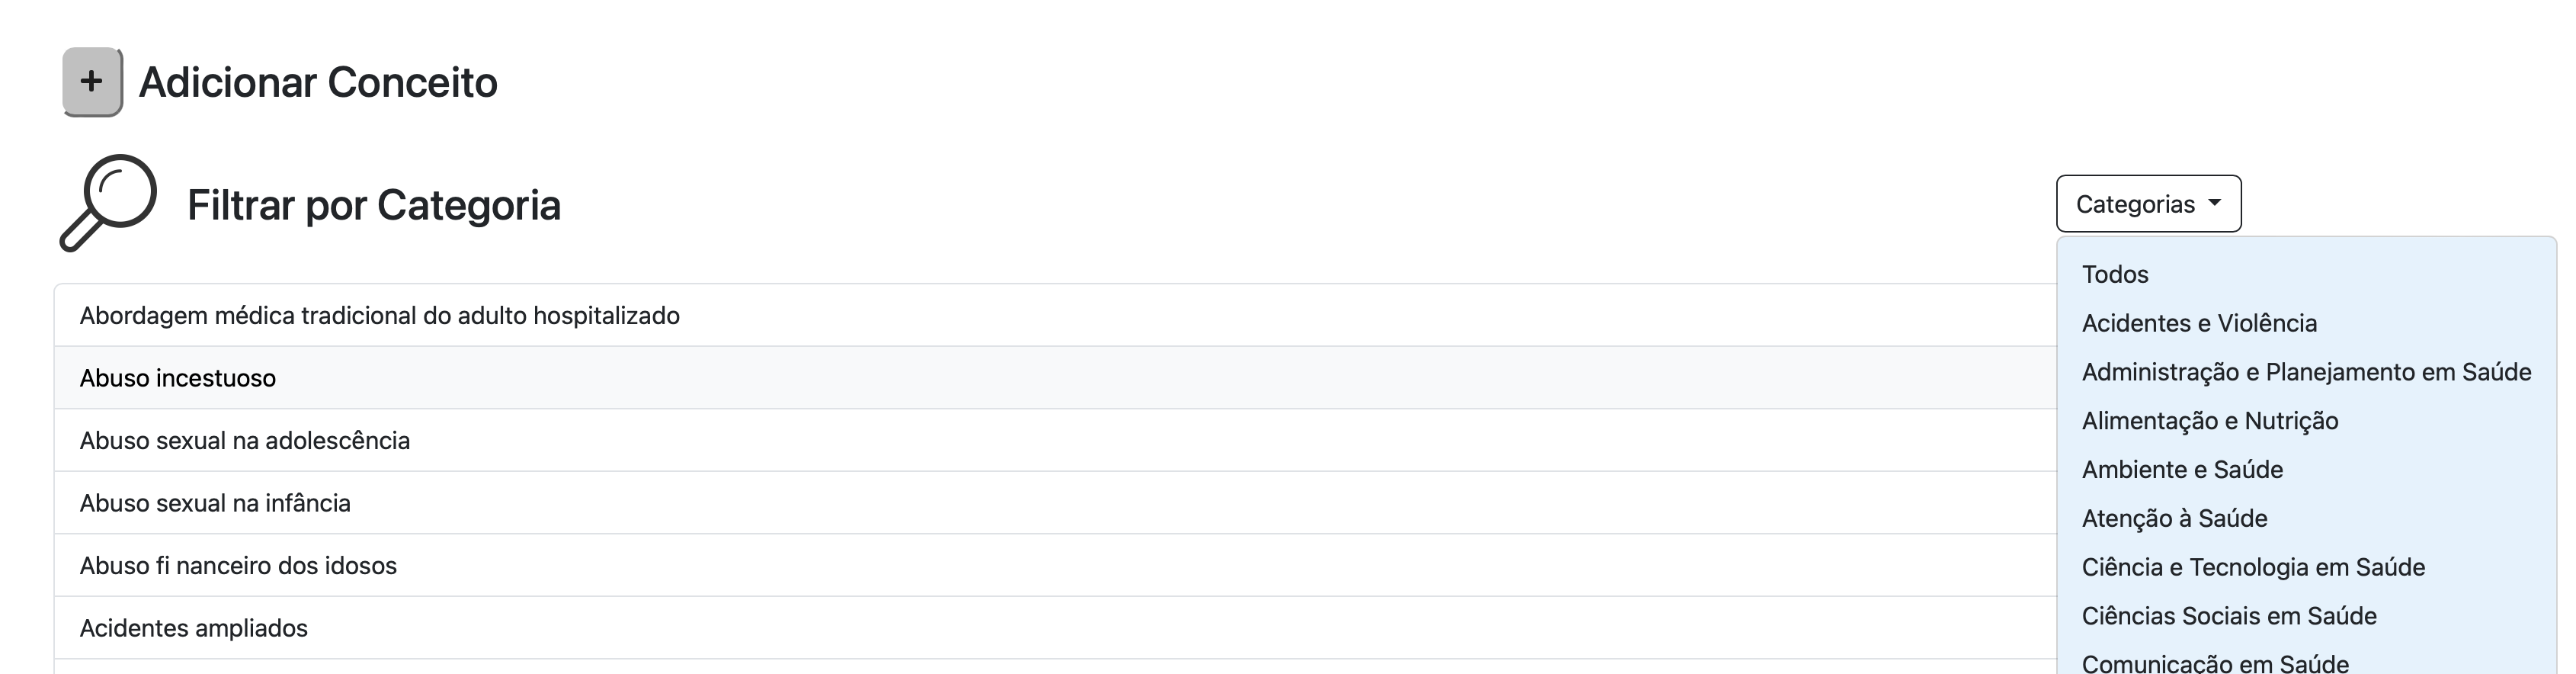
\includegraphics[width=0.9\textwidth]
    {Images/pagina_inicial_gloss.png}
    \caption{Página inicial da secção Glossário Global}
    \label{fig:dic-traduc1}
\end{figure}

\textbf{Adicionar novo conceito:}\\

O botão "Adicionar Conceito" presente na página inicial da secção Glossário Global permite o utilizador adicionar um novo conceito, que, ao ser pressionado, abre uma janela sobreposta à página.

Nesta janela, é possível selecionar, através de um \textit{dropdown menu}, para qual categoria o termo a ser adicionado é classificado e também preencher os campos relacionados à designação e à descrição. Assim como acontece para as outras secções do \textit{website}, não é obrigatória a adição da tradução dos termos em inglês. No entanto, caso seja de interesse do utilizador, com o uso de um \textit{toggle button}, é disponibilizado o elemento de \textit{input}, que permite a adição da tradução desejada.

\begin{figure}[H]
    \centering
    \centering
    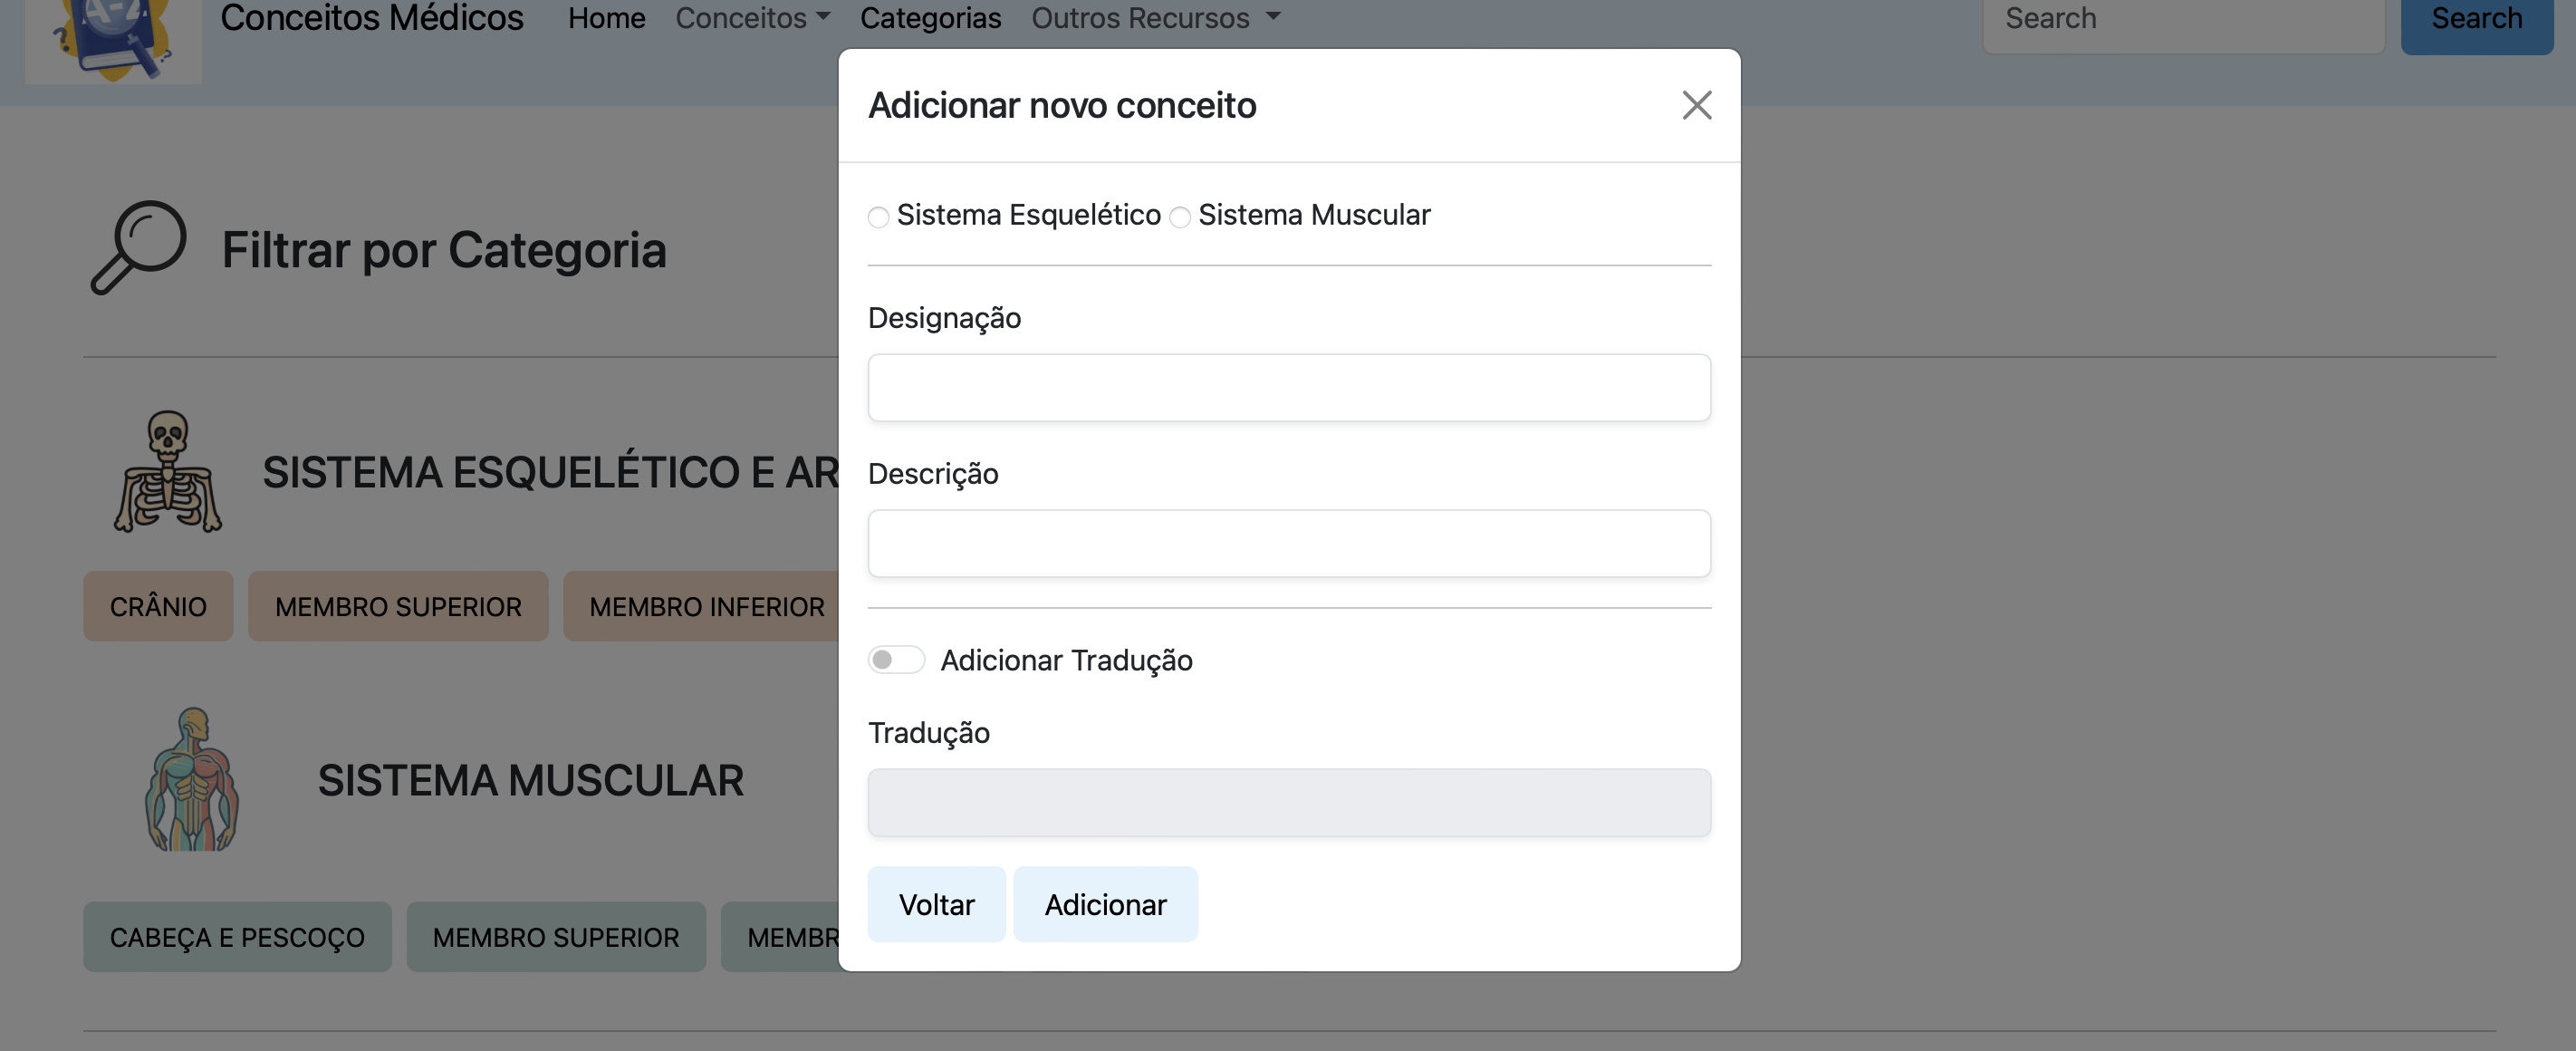
\includegraphics[width=0.9\textwidth]
    {Images/novo_glossario.png}
    \caption{Página inicial do Glossário Global com a janela sobreposta de adição de um novo conceito}
    \label{fig:dic-traduc1}
\end{figure}

 \newpage



